% The Plutus Platform Technical Report
% Note to contributors:
% - I am using a glossary package, as there is a *lot* of novel terminology in here.
%   Please use it as appropriate.
% - I am trying out a "precisely one sentence per line" policy (as opposed to reflowing with hard breaks) in an attempt to make diffs nicer.
%   Please also do so.
\documentclass{article}

\usepackage{amsmath, amssymb, stmaryrd, latexsym, mathtools}
\usepackage[hyperref]{ntheorem}

\usepackage[dvipsnames]{xcolor}
\usepackage{todonotes}
\usepackage{paralist}

% Smaller margins are nicer for this kind of content, I think.
\usepackage[margin=2.5cm]{geometry}

\usepackage{tikz}
\usetikzlibrary{arrows,shapes,snakes,automata,backgrounds,petri}

% TODO: better style
\usepackage[style=numeric]{biblatex}
\addbibresource{plutus.bib}

\usepackage{hyperref}
\hypersetup{
  breaklinks=true,
  colorlinks=true,
  urlcolor=NavyBlue,
  linkcolor=BrickRed,
  citecolor=Green
}

% Capitalize the "type" of the link, e.g. Section 2
\usepackage[capitalise]{cleveref}
% Automatically build the glossary index, and don't show the occurrence lists or add a dot at the end
\usepackage[automake, nonumberlist]{glossaries-extra}

\usepackage{fancyhdr}
\pagestyle{fancy}
\lhead{\color{red} DRAFT: DO NOT DISTRIBUTE}

\newcommand{\todompj}[1]{\todo[inline,color=yellow!40,author=Michael]{#1}}
% TODO: nicer code formatting inline and also in blocks
\newcommand{\code}[1]{\texttt{#1}}

% Break after header and don't italicise the body
\theoremstyle{break}
\theorembodyfont{\normalfont}

% An environment for requirements
\newtheorem{requirement}{Requirement}[section]

% cleveref "respects" your crefname and doesn't uppercase it even when
% capitalise is set, so you have to manually use their internal variable.
\makeatletter
\if@cref@capitalise
\crefname{requirement}{Requirement}{Requirements}
\else
\crefname{requirement}{requirement}{requirements}
\fi
\makeatother

% TODO: review the style
\setglossarystyle{altlist}
\makeglossaries
\setabbreviationstyle[acronym]{long-short-desc}
% General
\newglossaryentry{ada}{
  name=ada,
  description={
    The primary currency on the \gls{cardano} blockchain. Unlike other \glspl{currency}, ada cannot be forged.
  }
}
\newglossaryentry{cardano}
{
  name=Cardano,
  description={A third-generation blockchain developed by IOHK.}
}
\newglossaryentry{daedalus}
{
  name=Daedalus,
  description={The primary wallet frontend developed by IOHK for use with \gls{cardano}.}
}
\newglossaryentry{plutus-platform}
{
  name=Plutus Platform,
  description={
    The combined software support for writing \glspl{app}.
  }
}
\newglossaryentry{slot-leader}
{
  name=slot leader,
  description={
    The servers adding new blocks to the chain in the proof-of-stake Ouroboros protocol, corresponding to the miners of a proof-of-work protocol as employed in Bitcoin.
  }
}
\newglossaryentry{node}
{
  name=node,
  description={
    The user's local interface to the blockchain.
  }
}
\newglossaryentry{wallet-backend}
{
  name=wallet backend,
  description={
    The service that provides most of the wallet functionality, e.g. balance tracking, transaction submission, key management.
  }
}
\newglossaryentry{wallet-frontend}
{
  name=wallet frontend,
  description={
    A graphical user interface to a wallet, typically backed by a \gls{wallet-backend}, e.g. \gls{daedalus}.
  }
}

% Ledger
\newglossaryentry{address}{
  name=address,
  description={
    The address of an \gls{utxo} says where the output is ``going''.
    The address stipulates the conditions for unlocking the output.
    This can be a public key hash, or (in the \gls{eutxo-model}) a \gls{script} hash.
  }
}
\newglossaryentry{context}{
  name=context,
  description={
    A data structure containing a summary of the transaction being validated.
    See \cref{sec:eutxo}.
  }
}
\newglossaryentry{currency}{
  name=currency,
  plural=currencies,
  description={
    A class of \gls{token} whose \gls{forging} is controlled by a particular \gls{mps}.
  }
}
\newglossaryentry{currency-id}{
  name=currency id,
  description={
    An identifier for a \gls{currency}.
    This is the hash of the \gls{mps} that controls the \gls{forging} of the \gls{currency}.
  }
}
\newglossaryentry{data}{
  name=\textsf{Data},
  description={
    A generic type of structured data.
    See \cref{sec:data}.
  }
}
\newglossaryentry{datum}{
  name=datum,
  description={
    The data field on script outputs in the \gls{eutxo-model}.
    See \cref{sec:eutxo}.
  }
}
\newacronym[description={Our extended ledger model. See \cref{sec:eutxo}.}]{eutxo}{EUTXO}{Extended UTXO}
\newglossaryentry{eutxo-model}
{
  name=Extended UTXO Model,
  description={
    The ledger model which the \gls{plutus-platform} relies on.
    This is implemented in the Goguen release of \gls{cardano}.
    See \cref{sec:eutxo}.
  }
}
\newglossaryentry{forging}{
  name=forging,
  description={
    A transaction which forges \glspl{token} creates new \glspl{token}, providing that the
    corresponding \gls{mps} is satisfied.
    The amount forged can be negative, in which case the \glspl{token} will be destroyed instead of created.
    See \cref{sec:multicurrency}.
  }
}
\newglossaryentry{fungible}
{
  name=fungible,
  description={
    A \gls{token} is \emph{fungible} with another token if it can be used interchangeably with that token.
  }
}
\newglossaryentry{ledger}{
  name=ledger,
  description={
    A system for tracking ownership and transfers of assets.
    We will usually use this to mean ``distributed ledger''.
    See \cref{sec:ledger}.
  }
}
\newacronym[description={
  A \gls{script} which must be satisfied in order for a transaction to forge \glspl{token} of the corresponding \gls{currency}.
  See \cref{sec:multicurrency}.
}]{mps}{MPS}{Monetary Policy Script}
\newglossaryentry{multicurrency}
{
  name=multicurrency,
  description={
    A generic term for a ledger which supports multiple different currencies natively.
    See \cref{sec:multicurrency}.
  }
}
\newacronym[description={
  A unique token which is not \gls{fungible} with any other token.
}]{nft}{NFT}{Non-Fungible Token}
\newglossaryentry{one-shot}
{
  name=one-shot,
  description={
    A one-shot script is a script that requires that the pending transaction spend a specific existing transaction output.
    Since transaction outputs can only be spent once, this ensures that the script can only be (successfully) run once also.
    We may also refer to a one-shot transaction, which is a transaction that contains a one-shot script.
  }
}
\newglossaryentry{redeemer}
{
  name=redeemer,
  description={
    The argument to the validator \gls{script} which is provided by the transaction which spends a \gls{script-output}.
    See \cref{sec:eutxo}.
  }
}
\newglossaryentry{script}
{
  name=script,
  description={
    A generic term for an executable program used in the ledger.
    In the \gls{plutus-platform}, these are written in \gls{plutus-core}.
    See \cref{sec:eutxo}.
  }
}
\newglossaryentry{script-output}
{
  name=script output,
  description={
    A transaction output locked by a \gls{script}.
    See \cref{sec:eutxo}.
  }
}
\newglossaryentry{token}
{
  name=token,
  description={
    A generic term for a native tradeable asset in the ledger.
  }
}
\newglossaryentry{token-name}{
  name=token name,
  description={
    An identifier for a class of \glspl{token} within a \gls{currency}.
  }
}
\newacronym[description={
  A transaction output which has not been spent.
  Also refers to the traditional ledger model going back to Bitcoin.
}]{utxo}{UTXO}{Unspent Transaction Output}
\newglossaryentry{validator}
{
  name=validator script,
  description={
    The \gls{script} attached to a \gls{script-output} in the \gls{eutxo-model}.
    Must be run and return positively in order for the output to be spent.
    Determines the \gls{address} of the output.
    See \cref{sec:eutxo}.
  }
}
\newglossaryentry{value}
{
  name=\textsf{Value},
  description={
    A type representing a bundle of assets (\glspl{token}) in our \gls{multicurrency} system.
    See \cref{sec:value}.
  }
}

% Scripting
\newglossaryentry{cost-model}
{
  name=cost-model,
  description={
    A set of parameters which affect how the \gls{plutus-core} evaluator costs a program evaluation.
    See \cref{sec:costing}.
  }
}
\newglossaryentry{exunits}
{
  name=exunits,
  description={
    The units used to track execution costs.
    A pair of ``abstract time'' and ``abstract memory''.
    See \cref{sec:costing}.
  }
}
\newglossaryentry{plutus-core}
{
  name=Plutus Core,
  description={
    The programming language used for \glspl{script} in the \gls{plutus-platform}.
    See \cref{sec:plutus-core}.
  }
}
\newglossaryentry{system-f}
{
  name={\ensuremath{\textrm{System}\ F}},
  description={
    A well-known simple programming language, often called the ``polymorphic lambda calculus''.
  }
}
\newglossaryentry{system-fomf}
{
  name={\ensuremath{\textrm{System}\ F_{\omega}^\mu}},
  description={
    An extension of \gls{system-f} with recursive types and higher-kinded types.
  }
}

% Applications
\newglossaryentry{app}
{
  name=Plutus application,
  description={
    TODO: better name?
    An application built using the \gls{plutus-platform}.
  }
}
\newglossaryentry{app-api}
{
  name=contract API,
  description={
    TODO: better name?
    The interface provided by the \gls{paf} which \glspl{app} must use.
  }
}
\newglossaryentry{app-inst}
{
  name=application instance,
  description={
    A particular instance of an \gls{app}.
  }
}
\newglossaryentry{app-exe}
{
  name=application executable,
  description={
    The compiled executable from an \gls{app}.
  }
}
\newglossaryentry{chain-index}
{
  name=chain index,
  description={
    A component of the \gls{pab} that tracks information from the chain, notably output \glspl{datum}.
  }
}
\newglossaryentry{marlowe}{
  name=Marlowe,
  description={A domain-specific language for writing financial contract applications.}
}
\newglossaryentry{off-chain}
{
  name=off-chain code,
  description={
    The part of an \gls{app}'s code which runs off the chain, usually on a user's computer.
  }
}
\newglossaryentry{on-chain}
{
  name=on-chain code,
  description={
    The part of an \gls{app}'s code which runs on the chain (i.e. as scripts).
  }
}
\newacronym[description={
  The component which manages \glspl{app} run on users' machines.
  See \cref{sec:pab}.
}]{pab}{PAB}{Plutus Application Backend}
\newacronym[description={
  The overall framework for writing and running \glspl{app}.
  See \cref{sec:paf}.
}]{paf}{PAF}{Plutus Application Framework}

% Authoring
\newglossaryentry{ghc-core}
{
  name=GHC Core,
  description={
    GHC's internal representation of Haskell.
    A variant of \gls{system-f}.
  }
}
\newglossaryentry{plutus-ir}
{
  name=Plutus IR,
  description={
    An intermediate language that compiles to \gls{plutus-core}.
    See \cref{sec:plutus-ir}.
  }
}
\newglossaryentry{plutus-playground}
{
  name=Plutus Playground,
  description={
    A web based environment for trying out the \gls{plutus-platform}.
    See \cref{sec:plutus-playground}.
  }
}
\newglossaryentry{plutus-sdk}
{
  name=Plutus Haskell SDK,
  description={
    The libraries and development tooling for writing \glspl{app} in Haskell.
    See \cref{sec:sdk}.
  }
}
\newglossaryentry{plutus-tx}
{
  name=Plutus Tx,
  description={
    The libraries and compiler for compiling Haskell into \gls{plutus-core} to form the on-chain part of an \gls{app}.
    See \cref{sec:plutus-tx}.
  }
}



\begin{document}

\title{The Plutus Platform \\
  {\large \sc An IOHK technical report}}
\date{}
\author{
  Michael Peyton Jones \\ {\small \texttt{michael.peyton-jones@iohk.io}} \\
  \and Roman Kireev \\ {\small \texttt{roman.kireev@iohk.io}}
}

\maketitle

\tableofcontents

\section{Introduction}

Bitcoin, the most widely known and most valuable cryptocurrency, uses
a graph-based ledger model built on the concept of \emph{\UTXO{}s} (\emph{unspent
  transaction outputs})~\cite{formal-model-of-bitcoin-transactions,Zahnentferner18-UTxO}. Individual \emph{transactions} consist of a list of \emph{inputs} and a list of \emph{outputs}, where outputs represent a specific \emph{value} (of a cryptocurrency) that is available to be spent by inputs of subsequent transactions. Each output can be spent by (i.e., connect to) exactly one input. Moreover, we don't admit cycles in these connections, and hence we can regard a collection of transactions spending from each other as a directed acyclic graph, where a transaction with $m$ inputs and $n$ outputs is represented by a node in the graph with $m$ edges in and $n$ edges out.
The sum of the values consumed by a transaction's inputs must equal the sum of the values provided by its outputs, thus value is conserved.

Whether an output can be consumed by an input is determined by a function $\nu$ attached to the output, which we call the output's \emph{validator}. A transaction input proves its eligibility to spent an output by providing a \emph{redeemer} value $\rho$, such that \(\nu(\rho) = \true\) --- redeemers are often called \emph{witnesses} in Bitcoin. In the simplest case, the redeemer is a cryptographic hash of the spending transaction signed by an authorised spender's private key, which is checked by the validator, which embeds the corresponding public key. More sophisticated protocols are possible by using more complex validator functions and redeemers --- see \cite{bitml} for a high-level model of what is possible with the functionality provided by Bitcoin.

The benefit of this graph-based approach to a cryptocurrency ledger is that it plays well with the concurrent and distributed nature of blockchains. In particular, it forgoes any notion of shared mutable state, which is known to lead to highly complex semantics in the face of concurrent and distributed computations involving that shared mutable state.

Nevertheless, the \UTXO{} model, generally, and Bitcoin, specifically, has been criticised for the limited expressiveness of programmability achieved by the validator concept. In particular, Ethereum's \emph{account-based ledger} and the associated notion of \emph{contract accounts} has been motivated by the desire to overcome those limitations. Unfortunately, it does so by introducing a notion of shared mutable state, which significantly complicates the semantics of contract code. In particular, contract authors need to understand the subtleties of this semantics or risk introducing security issues (such as the vulnerability to recursive contract invocations that led to the infamous DAO attack~\cite{DAO-attack}).

\paragraph{Contributions.}

The contribution of the present paper is to propose an extension to the basic \UTXO{} ledger model, which
\begin{inparaenum}[(a)]
\item provably increases expressiveness, while simultaneously
\item preserving the dataflow properties of the \UTXO{} graph; in particular, it forgoes introducing any notion of shared mutable state.
\end{inparaenum}
More specifically, we make the following contributions:
%
\begin{itemize}
\item We propose the \emph{\EUTXO{} model}, informally in Section~\ref{sec:informal-eutxo} and formally in Section~\ref{sec:formal-model}.
\item We demonstrate that the \EUTXO{} model supports the implementation of a specific form of state machines (\emph{Constraint Emitting Machines}, or \CEM{}s), which the basic \UTXO{} model does not support, in Section~\ref{sec:expressiveness}.
\item We provide a formalisation of both the \EUTXO{} model
  and Constraint Emitting Machines. We prove a weak bisimulation
  between the two using the Agda proof
  assistant\site{https://github.com/\GitUser/formal-utxo/tree/\AgdaCommit}, building on
  previous work by Melkonian et al.~\cite{formal-eutxo}.
\end{itemize}

Section~\ref{sec:related} summarises related work.

The \EUTXO{} model will be used in the ledger of \Cardano{}, a major blockchain
system currently being developed by IOHK.
It also provides the foundation of Cardano's smart contract platform
\emph{Plutus}\site{https://github.com/input-output-hk/plutus}, which includes a small
functional programming language \emph{\Plutus{}} which is used to implement \script{}s.
Although a technical description of Cardano itself is beyond the scope of this paper,
one can try out the Plutus Platform in an online playground.\site{https://prod.playground.plutus.iohkdev.io/}

Other future work includes a formal comparison of \EUTXO{} with Ethereum's account-based model.

\iftoggle{anonymous}{
\paragraph{Anonymisation.}

For the purposes of submission, we have anonymised the following names:
\begin{itemize}
\item \Cardano{}: a major blockchain system.
\item \Plutus{}: a small functional programming language.
\end{itemize}
}{}

\section{The ledger: the Extended UTXO Model}
\label{sec:ledger}
\todompj{Maybe we should just move the content of the EUTXO doc into here?}

The \gls{plutus-platform} is designed to work with a specific kind of ledger, namely an extended form of the traditional \gls{utxo} ledger introduced by Bitcoin.
We refer to our ledger model as the \gls{eutxo} Model, and it is discussed in detail in \textcite{eutxo} and partially published as \textcite{chakravarty2020extended}.

We give a high-level overview here, further details can be found in the above references.

\subsection{Requirements}
\begin{requirement}[Locality]
\label{req:ledger-locality}
\Gls{utxo} ledgers have the nice property that all the information which is needed to validate a transaction is specified in the transaction.
All you need to check is the output that the transaction says that it spends.
In particular, there is no global state apart from the \gls{utxo} set.

This is in contrast to account-based ledgers, where account balances are global.

We aim not to disturb this property, since it is helpful in a number of ways.
For example, it allows a greater degree of parallel processing.
In \textcite{chakravartyhydra} this property is used to enable fast optimistic settlement of transactions off-chain, \emph{including} support for the scripting model we use.
This would not be possible if we followed Ethereum's actor model and had contract instances with global state.
\end{requirement}

\begin{requirement}[Determinism]
\label{req:ledger-determinism}
We would like our ledger rules to be \emph{deterministic}, that is, the outcome of transaction validation is entirely determined by the transaction in question (and the current state of the ledger of course).
This means that the whole process can be simulated accurately by the user \emph{before} submitting a transaction: thus both the outcome of validation and the amount of resources consumed can be determined ahead of time.
This is helpful for systems that charge for \gls{script} execution, since users can reliably compute how much they will need to pay ahead of time.

A common way for systems to violate this property is by providing \glspl{script} with access to some piece of mutable information, such as the current time (in our system, the current slot has this role).
\Glspl{script} can then branch on this information, leading to non-deterministic behaviour.
\end{requirement}

\begin{requirement}[Inspectability]
\label{req:ledger-inspectability}
As far as possible, we would like the data which we put on the ledger to be \emph{inspectable}.
Hence the \gls{off-chain} needs to be able to inspect the \gls{datum} and interpret it as a value it can work with.

This is primarily important for \gls{off-chain}.
For example, when implementing \glspl{app} which are state machines, we will use the \glspl{datum} of outputs to store the on-chain \emph{state} of the machine.
If the \gls{off-chain} wants to submit at transaction to advance such a state machine, it may need to read the current state from the chain (after all, the last transition might not have been performed by this agent).
\end{requirement}

\begin{requirement}[UTXO size]
\label{req:ledger-utxo-size}
\Glspl{slot-leader} are likely to be faced with resource constraints when doing transaction validation.
A key source of memory usage is that the whole set of current \gls{utxo} entries must be kept in memory at all times to check for double-spending.
Hence, it is important to keep the size of \gls{utxo} entries small.
\end{requirement}

\subsection{The \glsentryname{data} type}
\label{sec:data}

We will later require the ability to pass arguments to \glspl{script}.
However, this requires us to turn such arguments into values in our scripting language of the appropriate type.

We have opted to use a single, structured datatype for interchange with \glspl{script}.
We call this type \gls{data}, and it is described further in \textcite{eutxo}.\footnote{
  In practice it is very similar to other forms of structured data, such as JSON, but optimized to work with CBOR \autocite{cbor}.
}
This means that the \gls{redeemer} and \gls{datum} are of type \gls{data}, and the \gls{context} is encoded as \gls{data} before being passed to the \gls{validator}.

We also require a way to turn the \gls{data} values into values in our scripting language, but we can do this via the lifting machinery in \cref{sec:plutus-tx-lifting}.

On the user side, users are responsible for turning their specific types into \gls{data}, but this can be done in a standardized way, and we provide Template Haskell functions for generating the appropriate typeclass instances.

\subsection{UTXO ledgers}

A \gls{utxo} ledger represents a ledger as a series of \emph{transactions}, each of which has a set of transaction \emph{inputs} and transaction \emph{outputs}.

A transaction output carries some amount of \emph{value} and is \emph{locked} in some way that restricts how it can be spent.
The simplest form of locking is simply to attach a public key.

A transaction input is a reference to a transaction output.
For example, a pair of a transaction ID and an index into the (ordered) set of its outputs.

\subsubsection{UTXO validity}
\label{sec:utxo-valid}

For a transaction to be \emph{valid} against an existing \gls{utxo} ledger, it must be the case that:
\begin{itemize}
\item All inputs refer to outputs which exist in the ledger and have not been spent by another transaction in the ledger.
\item The transaction balances: the sum of the value on the spent outputs equals the sum of the value on the transaction outputs.
\item The transaction is authorized: for each spent output locked by a public key, the transaction contains a witness (a signature over the transaction body) from the corresponding private key.
\end{itemize}
\medskip

Hence ownership in a \gls{utxo} ledger consists in having the right to spend an output: one owns outputs rather than an aggregate amount of funds.

\subsection{EUTXO-1: scripting}
\label{sec:eutxo}

\todompj{This section is a mess and doesn't tell the story well.}

The first addition we make is to support scripting.
Our approach is based of existing models for \gls{utxo} ledgers with scripts (e.g. \textcite{Zahnentferner18-UTxO}), but we make a number of additions.

We make the following changes to the \gls{utxo} model:

\begin{itemize}
\item
  Every transaction has a \emph{validity interval} over slots.
  A \gls{slot-leader} will only process the transaction if the current slot number lies within the transaction's validity interval.

\item
  The ledger learns about a \emph{scripting language} and how to evaluate scripts in that language.\footnote{
    In the \gls{plutus-platform} this language is \gls{plutus-core}.
    }

\item
  Transaction outputs can be locked by a \gls{validator} (such outputs are called \glspl{script-output}).

\item
  \Glspl{script-output} have an attached \gls{datum}, which is a value of type \gls{data}.

\item
  When spending a \gls{script-output}, the spending transaction must provide a \gls{redeemer} of type \gls{data} for each such output.

\item
  Validator scripts are passed three arguments: the \gls{datum} of the output being spent, the \gls{redeemer} for the output, and a value called the \gls{context} which has a representation of the transaction being validated.
\end{itemize}

\todompj{I'm totally glossing over the details about which things are hashes and the whole data witnesses thing.}

\subsubsection{The contents of the context}
The \gls{context} type is a summary of the information contained in a transaction, made suitable for consumption in a \gls{script}.

The exact form is subject to change (see \textcite{eutxo} for the details), but it should contain all the information about the inputs, outputs, metadata, etc.

\subsubsection{Ensuring determinism}
The information provided by the \gls{context} is entirely determined by the transaction itself.
This ensures that we satisfy \cref{req:ledger-determinism}.

We handle the issue of time by providing only the validation interval of the transaction.
This serves to give the \gls{validator} a window within which the current time must lie: in practice this is enough to establish that the current time is ``definitely before'' or ``definitely after'' some particular time, which is the most common kind of constraint.

Some additional responsibility passes to the author of the transaction as a result of this.
If the \gls{validator} they are trying to satisfy requires that the transaction occur before some time $T$, then they must not only submit the transaction before $T$, they must ensure that the upper bound of the validity interval is below $T$.
This doesn't make the transaction less likely to validate (it would not have validated after $T$ regardless!), but it does require some more work from the \gls{off-chain}.

\subsubsection{EUTXO-1 validity}
\label{sec:eutxo-1-valid}

In addition to the conditions in \cref{sec:utxo-valid}, the following condition must hold:
\begin{itemize}
\item Scripts must succeed: if a transaction spends a \gls{script-output}, then the \gls{validator} on the output must be run with the \gls{redeemer}, \gls{datum}, and \gls{context} and return successfully.
\end{itemize}

\subsection{EUTXO-2: \glsentrytext{multicurrency}}
\label{sec:multicurrency}

\todompj{This section is also a mess and doesn't tell the story well.}

The other extension that we make to the ledger is to enable \emph{\gls{multicurrency}}, that is, to enable our ledger to represent a wider variety of assets than a single one.
\Gls{multicurrency} is a key part of the \gls{plutus-platform} not only because custom \glspl{currency} are an important use case for blockchain systems, but because we use lightweight custom \glspl{token} as integral parts of our application designs.

The key design innovation is that \glspl{currency} are identified with the hash of the \gls{mps} that controls them.
This means that to be allowed to forge \glspl{token} of a particular \gls{currency}, you must present the corresponding \gls{mps} with the transaction and it must pass.

This design allows our system to be both \emph{local} and \emph{lightweight}:
\begin{itemize}
\item
  We do not require any kind of central registration of \glspl{currency}: any hash can be used as a \gls{currency-id}, you just cannot forge any unless you can produce a \gls{script} with that hash.
  This ensures we do not violate \cref{req:ledger-locality}.
\item
  \Gls{forging} \glspl{token} is cheap: all that is required is to provide and run the script at the time of forging.
\item
  Transacting with custom \glspl{currency} is cheap: they are natively supported and work just like the native token.
\end{itemize}

\todompj{Say more, maybe write out some of the requirements separately.}

\subsubsection{The \glsentryname{value} type}
\label{sec:value}
The first change we make is to our notion of ``value'' on the ledger.
In traditional \gls{utxo} ledgers, value is just an integer representing a quantity of the (unique) asset tracked by the ledger.

We generalize this to support multiple asset classes as follows: we define a type \gls{value} which represents a \emph{bundle} of assets, indexed by a \emph{\gls{currency-id}} and then by a \emph{\gls{token-name}}.

\begin{quote}
\begin{verbatim}
type Value = Map CurrencyID (Map TokenName Quantity)
\end{verbatim}
\end{quote}

The \gls{currency-id} indicates the \emph{controller} of the currency, specifically it is the hash of the \gls{mps} that controls when tokens of that currency may be forged or destroyed (see \cref{sec:forging}).
The \gls{token-name} separates different \emph{classes} of \gls{token} within the currency. Only \glspl{token} of the same currency and \gls{token-name} are \gls{fungible} with each other.
Hence one could use a currency to track items in a game: different kinds of items would have different \glspl{token-name}, and an asset bundle could consist of e.g. 3 swords, 7 hats, and a cheesecake.

Operations on \gls{value} are defined as if it were a finitely-supported function.

The ledger rules do not need to change much in order to support this generalized the \gls{value}: the only change is that we need to use the appropriate sum operation on \gls{value} in e.g. the balancing rules.

\subsubsection{\Glsentrytext{forging}}
\label{sec:forging}
\Gls{value} may also be created and destroyed, we call this \emph{\gls{forging}}.
To this end transactions are given two additional fields:
\begin{enumerate}
\item \code{forge} which contains \gls{value}
\item \code{forgeScripts} which contains \glspl{mps} for all the \glspl{currency} forged in \code{forge}
\end{enumerate}

\subsubsection{\glsentrylong{mps}s}
The \glspl{script} which control the forging of \glspl{token} are called \glsfirstplural{mps}.
Since these are able to see the \gls{context}, and hence the whole transaction being validated, they can enforce a wide range of properties on the transaction.

\subsubsection{\glsentrylong{nft}s}
A \gls{nft} is a unique \gls{token} which can be transferred to another user, but not duplicated.
\Glspl{nft} have proven useful in a number of blockchain applications (see \textcite{ERC-721}); for example, they can represent ownership of some object in a game, or shares in a company, or many other kinds of asset.
We can implement \glspl{nft} as token classes within a \gls{currency} whose supply is limited to a single \gls{token}.

Ensuring that the tokens are unique is not trivial, since uniqueness is a global property and transactions only have access to local information.
Two approaches are:
\begin{itemize}
\item
  Use a \gls{one-shot} \gls{mps}.
  This ensures that the \gls{mps} can only be run once, and then so long as you do not issue any duplicates there, you will have uniqueness.
\item
  Run a unique state machine (beginning with a \gls{one-shot} transaction to ensure uniqueness) which keeps all the issued tokens in its state.
  This effectively introduces global state that must be consulted before each forging, allowing uniqueness to be maintained.
\end{itemize}

\subsubsection{EUTXO-2 validity}
\label{sec:eutxo-2-valid}

In addition to the conditions in \cref{sec:utxo-valid} and \cref{sec:eutxo-1-valid}, the following condition must hold:
\begin{itemize}
\item Forging must be authorized: for each \gls{currency-id} of which a non-zero amount is forged in \code{forge}, the corresponding \gls{mps} must be run with the \gls{context} and return successfully.
\end{itemize}

\section{Scripting: Plutus Core}
\label{sec:plutus-core}

Our scripting language for the \gls{plutus-platform} is \gls{plutus-core} (strictly, type-erased \gls{plutus-core}, see \cref{sec:erasure}).
A formal specification for \gls{plutus-core} is available in \textcite{plutus-core-spec}.

We give a high-level overview of the language here, further details can be found in the above reference.

\subsection{Requirements}
\begin{requirement}[Conservatism]
\label{req:script-lang-conservatism}
Designing a new programming language is hard.
It is very easy to make choices that come back to haunt you.

Moreover, whatever language we choose for our scripting language will be very hard to change, since it will be involved in transaction validation, and we want to be able to validate old transactions.
So we can release new versions, but we must support old versions forever.

This combination means that it is hard for us to get the language right first time, and it is also hard for us to iterate on it.
This suggests a case for \emph{conservatism}: pick things that are tried and tested, and don't try to innovate too much.

Conservatism also makes requirements such as \cref{req:script-lang-formalization} easier to satisfy, as we can build on existing work.
\end{requirement}

\begin{requirement}[Minimalism]
\label{req:script-lang-minimalism}
The smaller our language, the less there is to go wrong, and the less there is to reason about.

Minimalism makes requirements such as \cref{req:script-lang-formalization} easier to satisfy, since there is less to formalize.

However, this is a tradeoff, as a simpler target language often means more complexity in the compilers that target that language.
But it is much easier for us to change the compilers than it is to change the scripting language, so this is worth it.
\end{requirement}

\begin{requirement}[Safety]
\label{req:script-lang-reasoning}
Once submitted as part of a blockchain transaction, scripts are immutable.
Therefore we want as much certainty as we can get about what the code will do, otherwise there is risk that the value involved will be lost or stolen.
\end{requirement}

\begin{requirement}[Formalization]
\label{req:script-lang-formalization}
One part of reasoning about what our programming language does is to \emph{formalize} its semantics, so we can be sure that
\begin{inparaenum}
  \item it has a sensible semantics, and
  \item the implementation agrees with that semantics
\end{inparaenum}.
\end{requirement}

\begin{requirement}[Size]
\label{req:script-lang-size}
The representation of the scripting language on the chain must not be too large, since
\begin{inparaenum}
\item users will pay for the size of transactions, and
\item transaction size has a major effect on the throughput of the system.
\end{inparaenum}
\end{requirement}

\begin{requirement}[Extensibility]
\label{req:script-lang-extensibility}
We may want to use our scripting language on other ledgers in the future, and they may well support different basic primitives, so we need this to be configurable.
For example, privacy-preserving ledgers may restrict the kinds of computation that can be done, which may mean we only have some kinds of arithmetic operations.
\end{requirement}

\begin{requirement}[Multiple source languages]
\label{req:source-lang-multiple}
It would be nice if multiple source languages could be compiled to our scripting language.
This would potentially encourage usage by developers who are more comfortable with one or the other of the source languages.

However, this is somewhat speculative and actually implementing other source languages would be a lot of work.
But if we can cheaply make this easier then that is good.
\end{requirement}

\subsection{Designing Plutus Core}

How do we design our scripting language?
\Cref{req:script-lang-conservatism,req:script-lang-minimalism} suggest adhering to existing languages as much as possible, and picking a small, well-studied language.
We also want to use a statically-typed functional programming language, since we intend to use functional programming languages (starting with Haskell) as our source languages.

This suggests using some variant of the lambda calculus.
We decided to start with \emph{\gls{system-f}}, also known as the polymorphic lambda calculus \autocite{Girard-thesis}.
Haskell's internal language, \gls{ghc-core} \parencite{jones1998transformation}, is also based on \gls{system-f} (no coincidence), but we make a couple of different decisions:
\begin{enumerate}
  \item We do not have primitive datatypes and case expressions, rather we base our language on \emph{\gls{system-fomf}}, which extends \gls{system-f} with recursive types and higher-kinded types.
  \item Our language is strict, rather than lazy, by default.
  \item We do not support most of the extensions that Haskell has pioneered, such as coercions.
\end{enumerate}

As a result, the formal specification of our language can be described in one line: it is exactly \gls{system-fomf} with appropriate primitive types and operations.


\subsection{Datatypes}
If we do not have primitive datatypes, how \emph{do} we deal with datatypes?
The answer is that it is up to the compiler to encode them --- another example of the tradeoff discussed in \cref{req:script-lang-minimalism}.

In our case \gls{plutus-ir} does have datatypes, so this is handled by the \gls{plutus-ir} compiler. See \cref{sec:plutus-ir} for more details.

\subsection{Recursive types}

The one-line description above turns out not to be as unambiguous as one might hope. We have
to choose between equirecursive types and isorecursive types \autocite[chapter 21]{pierce2002types}.

There is a tradeoff here between simplicity of writing code in the language, and simplicity of the language's metatheory.
Since \gls{plutus-core} is a compilation target rather than a source language, we opted to go for isorecursive types, which have the simpler metatheory (aiding \cref{req:script-lang-formalization}).
The complexity is handled by the \gls{plutus-ir} compiler.

This choice is discussed more in \textcite{plutus-core-spec, peytonjones2019unraveling}.

\subsection{Recursive values}

While \gls{plutus-core} has support for recursive types, it does not have any (direct) support for recursive \emph{values}.
It turns out that recursive types are sufficient to implement the usual array of fixpoint combinators, and so encode recursive values \autocite{harper2012practical}.
Again, this encoding is handled by the \gls{plutus-ir} compiler, see \cref{sec:plutus-ir}.

Doing this in full generality turns out to be surprisingly tricky, see \textcite{peytonjones2019unraveling}.

\subsection{Builtin types and values}

Programming languages commonly have some form of foreign function interface. The idea is that:

\begin{enumerate}
\item
  We don't want to reimplement everything from the bottom up in a newly designed language.
  It makes much more sense to delegate certain computations to an existing tool where such computations already exist in optimized form, with good tests etc.
\item
  In particular, We certainly don't want to implement our own version of arithmetic (integers, addition, multiplication, etc.) or any other low-level stuff where it will be especially hard to beat external implementations.
\end{enumerate}

We certainly need efficient primitives in \gls{plutus-core}, including arithmetic.

To implement this, we could build \code{Integer} into the grammar of \gls{plutus-core} types, and \code{Integer} constants into the grammar of \gls{plutus-core} terms, as well as a few functions (addition, multiplication, etc.).
If we need more types or functions, then we simply have to extend the hardcoded list of types and functions.

However, this is very inflexible.
The key issue is that we may want to have \emph{different} sets of builtins in different situations.
For example:
\begin{enumerate}
\item
  During testing it can be convenient to have a builtin which implements \emph{tracing}: emitting log lines to a global trace output.
  But we don't want this functionality on-chain, so we want to remove the builtin (or replace it with a no-op).
\item
  We may need different builtins for different ledgers (see \cref{req:script-lang-extensibility}).
\end{enumerate}

So we need to make builtin types and functions extensible.

\subsubsection{Builtin types}

Extensible builtin types are relatively straightforward on the type level where they are opaque --- we don't need to know anything about a type other than its kind in order to handle type normalization etc.
However, values of builtin types (``constants'' in \gls{plutus-core}) are trickier.
It's easy to say what a \code{Integer} constant should be: an integer!
However, what about constants of extensible builtin types?

We adopt an approach familiar from generic programming in dependently-typed languages, where we use a \emph{universe} of types to represent the types our programs can operate over.\footnote{
  Where do these types themselves come from?
  We assume that we are working in some ``metalanguage'' which has types such as \code{Integer} that we can reuse in Plutus Core.
}
In our case, we are entirely parametric over the universe itself, with different universes corresponding to different sets of builtin types.
A constant then is then \emph{tagged} with a value corresponding to a type in that universe, and a value of that type.

This does complicate interpretation of \gls{plutus-core} programs, since in order to interpret a program, you also need to know what universe of types it is expecting.
In practice this is not so bad: for most users (e.g. the \gls{cardano} ledger) there will be a single universe that they use, and from there on they can simply act as though we did not have extensible builtins.

\paragraph{Builtin datatypes}

Adding new types to \gls{plutus-core} is not very useful unless they have functions that can operate on them!
A particularly common case is where the new type is a datatype, and should support pattern matching.
We can support this by also providing a ``matching'' function as a builtin function.\footnote{
  These functions look just like the ``matchers'' for Scott-encoded datatypes, which is no coincidence.
}

For example, the matching function for \code{bool} is \code{ifThenElse :: forall a . bool -> a -> a -> a}.
Matching functions are always polymorphic, which is a key reason why we need to support polymorphic builtin functions (see \cref{sec:polymorphic-builtins}).

\paragraph{Polymorphic builtin types}

It would be nice to support polymorphic builtin types.
For example, that would allow us to provide optimized implementations of container types such as maps.

This seems feasible in principle, but we have not worked the details out yet.

\subsubsection{Builtin functions}

We could implement extensible builtin functions in a similar way to extensible builtin types: use some type (like the universe for types) that catalogues the available builtin functions.
However, in practice we don't need to model the available functions quite as precisely, since the syntax doesn't depend on the available functions as it does on the available types.

So instead we adopt a much simpler approach where the available builtin functions can be provided at runtime simply indexed by a name.
We may change this in future to use the explicit catalogue of functions.

\paragraph{Passing arguments to builtin functions}

Builtin functions must of course be provided with a type signature (since we have a typed language), and a way to evaluate them.
The natural way to provide such evaluators is as functions --- but these functions must be able to operate on \gls{plutus-core} terms!
For example, an evaluator for ``plus'' must be able to take two \emph{terms} of type \code{Integer} and turn them into another term.
But a simple implementation of ``plus'' just talks about \emph{integers}, not terms.

Solving this problem in generality is difficult, so we make a key simplification: builtin functions may only accept arguments of builtin types (with one exception, as we will see shortly).
Along with the fact that (since \gls{plutus-core} is eager) function arguments are evaluated to values before being passed to the function, this means that the arguments to builtin evaluators will always be \emph{constants}, which are easy to unwrap into their underlying values.

\paragraph{Polymorphic builtin functions}
\label{sec:polymorphic-builtins}

The exception to the above rule about builtin function types is for \emph{polymorphic} builtin functions.
These must necessarily be able to process arbitrary terms (since they can be instantiated at any type, not just a builtin type).
For example, \code{ifThenElse} must be able to produce a value of type \code{Integer -> Integer}, even though this is not a builtin type.

It is possible in principle to use polymorphic \emph{evaluators} to implement polymorphic builtin functions \autocite{lindley2012embedding}.
Unfortunately this is quite a heavyweight and complex encoding for such a key usecase.

Instead, we require evaluators for polymorphic functions to be \emph{parametric}, which means in particular that they do not inspect their polymorphic arguments.
We can thus pass the \emph{term itself} as the polymorphic argument, instead of needing to extract a value of an appropriate type in the metalanguage, as we do for other arguments.
Thus, an evaluator for a builtin function which implements \code{const :: forall a b . a -> b -> a} would take two \emph{terms} and return the first one.

\paragraph{Saturated builtin application}

When including builtin function application in the AST, we have two options:
\begin{enumerate}
\item
  Builtin functions can stand alone as a value with the builtin's function type, and are applied to their arguments with normal function application.
\item
  Builtin functions must always appear \emph{saturated}, that is, with all of their arguments.
\end{enumerate}

There choice is fairly minor, but has a few consequences:
\begin{enumerate}
\item
  Unsaturated builtins can be partially applied, saturated builtins cannot be --- but we can easily work around this by wrapping the builtin in a lambda, so this does not matter in practice.
\item
  Saturated builtins are easier to write an efficient evaluator for.
  Unlike normal functions, we cannot do any real evaluation of a builtin function until we have \emph{all} the arguments.
  So it is easier if we only ever see them with all their arguments.
\end{enumerate}

We've chosen to use saturated builtin applications.

\paragraph{Errors from builtin functions}

Builtin functions \emph{are} currently allowed to fail, i.e. to use the \code{error} effect in \gls{plutus-core}.
This allows us to handle cases like $1 \div 0$ without having to complicate the builtin machinery with an explicit error handling facility like \code{Maybe}.

Builtin functions are \emph{not} currently allowed to catch errors (nothing in \gls{plutus-core} can catch an error, currently).

\subsection{Erasure}
\label{sec:erasure}

Originally we planned to use typed \gls{plutus-core} as the actual scripting language.
However, we discovered that the explicit types made up a large proportion of the overall size of the code ($\approx 80\%$).
Given that we care about size (\cref{req:script-lang-size}), this was too compelling an improvement to pass by.

Hence we decided to instead use \emph{type-erased} \gls{plutus-core} as our scripting language instead, with typed \gls{plutus-core} as a (useful) intermediary language.

We were initially concerned that if we did not typecheck the application of the \gls{validator} to its arguments (which we cannot do if we've erased the types of the \gls{validator}!), then that might allow a malicious attacker to pass a script ill-typed arguments, potentially causing unexpected behaviour.
However, given the current design where all the arguments to the \gls{validator} are of type \gls{data}, and are constructed by the validating node (which is a trusted party), it is no longer possible for the arguments to be ill-typed.

Erased \gls{plutus-core} is much closer to the untyped lambda calculus, and as such is also an easier compilation target (e.g. for a dependently-typed language, or a non-statically-typed language), hence this also helps with \cref{req:source-lang-multiple}.

\subsection{Formalization}

As discussed in \cref{req:script-lang-formalization}, we would like to formalize \gls{plutus-core}.
We have done so in Agda: the resulting formalization is partially published in \textcite{chapman2019system}, and the living version is available in \textcite{plutus-repo}.

Our formalization includes the type system and semantics, proofs of progress and preservation, and an evaluator which provably implements the semantics.
This evaluator can be extracted to a Haskell executable, which we use to cross-test against the Haskell interpreter.

\section{Resources: Costing Plutus Core}
\label{sec:costing}

A key, unusual, requirement of the scripting language we use is that it must have a built-in notion of resource tracking.
We are going to run untrusted code on many machines during transaction validation and diffusion - it is important that we carefully control its resource usage.

This is a familiar problem in other systems such as Ethereum (which tracks resource usage using ``gas''), but we are focussing on a somewhat different set of requirements.

\subsection{Requirements}
\begin{requirement}[Profitable fees]
\label{req:costing-profitability}
\Glspl{slot-leader} are compensated for the work that they do to validate transactions by being given the transaction fees.
This ensures that it is economical (or even profitable) to run a stake pool even just based on transaction fee income.
We, therefore, need to ensure that the fees for script execution don't change this dynamic, e.g. by making it un-economical to run a pool.

If transactions with scripts are un-economical to process, then slot leaders may simply choose not to include them, which would compromise the usability of the system.
\end{requirement}

\begin{requirement}[DoS security]
\label{req:costing-dos}
Scripts allow the user who submits a transaction to force every node on the network to perform some computation of the user's choice.
This provides an obvious angle for DoS attacks: simply flood the network with pointless transactions that require a lot of computation, thus preventing the network from doing anything else.
Of course, any such attack must pay the script execution fees for these transactions.
So we need to make the fees high enough that such an attack is un-economical.
\end{requirement}

\begin{requirement}[Usable fees]
\label{req:costing-usable}
We do want users of \gls{cardano} to actually use scripts.
So the cost to run scripts can't be too high, otherwise, nobody will use them.
The simplest way to encourage this is to make the evaluator faster, which benefits legitimate users without compromising the security of the system.
\end{requirement}

\begin{requirement}[Determinism]
\label{req:costing-determinism}
Script execution cost affects whether a transaction validates, and as such if the costs are non-deterministic then it is non-deterministic whether a transaction with scripts will validate at all.
Predictable costs ensure that users can submit transactions and be sure that they will validate (or if they don't, it will be for other reasons).

See also \cref{req:ledger-determinism}.
\end{requirement}

\begin{requirement}[Evaluator abort]
\label{req:costing-abort}
The evaluator must be able to run scripts with limited resources and stop when they exceed them, so we actually enforce budgets.
\end{requirement}

\begin{requirement}[Intuitive costs]
\label{req:costing-intuitive}
Programmers will want to reason about costs when writing their programs.
So ideally costs should track those intuitions.
That way, if a user does something that they expect to reduce the cost of the program, then it probably does do so.
\end{requirement}

\begin{requirement}[Specifiablity]
\label{req:costing-specifiable}
We want to formally specify how the costs for a script should be calculated, which means that the method for computing them must be relatively simple and manageable to specify.
\end{requirement}

\begin{requirement}[Low overhead]
\label{req:costing-overhead}
Tracking costs during script execution should not impose too much overhead.
We don't want the process of preventing scripts from running too slow to itself slow them down significantly!
\end{requirement}

\begin{requirement}[Parameterizable models]
\label{req:costing-parameters}
We are unlikely to get all the numeric choices about how to assign costs correctly the first time.
Or, they might be invalidated by hardware or software changes.
Hence we should parameterize the model so that the ledger can change the parameters (e.g. with a protocol parameter update).
\end{requirement}

\begin{requirement}[Language-agnostic ledger support]
\label{req:costing-language-agnostic}
The ledger will support many different languages, which may think about costing in quite different ways.
We want to make this as easy as possible, ideally by abstracting away some of the details.
\end{requirement}

\begin{requirement}[Block budgets]
\label{req:costing-block-budget}
We have some constraints on how long block validation as a whole can take, in order to ensure that blocks can propagate across the network fast enough.
In addition, we have limits on how much peak memory we can use in a block, based on our expectations of typical hardware.

We may therefore need hard limits on resource usage per-block, in addition to setting prices for resource usage.
\end{requirement}

\subsection{Non-Requirements}
There are some things which we could have designed for but we have chosen not to.
A few notable examples are given here.

\paragraph{Units of cost should be persistent across transactions}
On Ethereum, the gas which a contract does not spend in a single transaction is persistent - it can be used later.
We don't intend to replicate this: because execution costs are predictable, it is no problem to require users to provide exactly the amount that they need.
Moreover, persistent cost units potentially allow undesirable arbitrage where a user can ``buy'' computation when it is cheap and ``spend'' it later when it is expensive, which is not what the network wants.

\paragraph{Users should be able to calculate script execution costs for any input to that script}
Users often care about the ``total cost of operation'' of an application.
But this may consist of running the same script with many different inputs across time, depending on contingent facts which will not be known until later.
To give this information to users precisely we would need to be able to predict, for any input, what the execution cost would be.
This is something that has been studied, but we believe it would be a lot of work to apply to our situation.
\footnote{
  There is research in doing this for languages with explicit recursion and datatypes.
  We would probably want to do this analysis on Plutus IR, and then try and translate the analysis down to Plutus Core.
  This seems like a substantial amount of work, probably a PhD thesis or so.
}
Users will still be able to get some idea of total cost of operation by running their script with a selection of indicative inputs.

\paragraph{Slot leaders should be compensated for the opportunity cost of memory usage}
We want to enforce a peak memory limit to avoid crashes, but we don't bother compensating slot leaders for the opportunity cost of using their memory.

\subsection{High-level approach}
This section gives a very high-level overview of the approach we take to the problem.
Further details on each of these topics are given later.

\paragraph{Abstract resources}
Rather than computing costs directly in Ada or in real resource units (e.g. seconds), we instead compute them in \emph{abstract resource units}, which do not have a definitional link to real resources.
The reasons for this are that:
\begin{itemize}
\item Costs must be deterministic and specifiable (\cref{req:costing-determinism,req:costing-specifiable}), so we cannot use \emph{real} resource units that will differ by machine.
\item The decision for how to convert these resource units into Ada (``pricing'') can be the ledger's responsibility alone.
\item Language-specific costing solutions don't need to worry about the (potentially strategic) concerns that affect pricing (\cref{req:costing-language-agnostic}).
\end{itemize}

\paragraph{Limiting execution}
The evaluator can run in a mode (``restricting'') where it is given a budget of abstract resources and terminates if the execution exceeds that (\cref{req:costing-abort}).
We also provide another mode (``counting'') where we do not receive a budget, and instead return the minimum budget that the script requires.

\subsubsection{Cost model}
We call the system which tells the evaluator how much an script should cost a ``cost model''.

\paragraph{Cost model strategy}
The cost model for \gls{plutus-core} is defined in a fairly simple, compositional way by giving costs for individual operations and then accumulating them over the course of the evaluation.

This cost model naturally has a lot of parameters: the numbers that influence the costs for the individual operations.
We allow all of these to be changed, so the evaluator accepts a bag of parameters that gives all of these values.
These parameters will be put into the protocol parameters, so we should have a large amount of flexibility if we need to tweak the cost model later (\cref{req:costing-parameters}).

\paragraph{Choosing the cost model parameters}
The decoupling of the abstract resource units from the pricing units allows us to use a fairly simple rubric for picking cost model parameters: try and actually follow (be correlated with) real costs!

This ensures that resource costs will follow programmers' intuitions (\cref{req:costing-intuitive}), while giving plenty of flexibility in the final pricing of those resources.

If we later change our minds about the cost model parameters (e.g. because what we consider ``typical hardware'' changes), we can re-calibrate our parameters and submit a protocol parameter change.

However, we do want our choices to generally be an \emph{over-approximation} because anywhere we under-approximate is a potential source of attacks (\cref{sec:costing-security}).

\subsubsection{Pricing model}
The conversion from abstract resources to Ada is done by the ledger.
We call the system which tells us how to do this conversion the ``pricing model''.

\paragraph{Pricing model strategy}
The current proposed pricing model simply consists of an Ada price for each of the abstract resources.
So a budget in terms of \gls{space} and \gls{time} will be turned into a price in terms of Ada by multiplying the components of the limit by their respective prices.

These prices also obviously function as parameters for the pricing model.
Hence they will also be put in the protocol parameters, so that pricing can be changed with only a protocol parameter change.

\paragraph{Choosing the pricing model parameters}
Choosing the pricing model parameters is a complex problem that may have strategic considerations.
At a minimum, the prices will need to be high enough to avoid DoS attacks (\cref{req:costing-dos}).

\subsubsection{Validating scripts}
Putting the pieces together, what happens when a script is validated is:
\begin{itemize}
\item
  The ledger uses the pricing model parameters to compute the price for the stated resource budget in Ada and ensures that the transaction has sufficient fees to cover this and that it does not cause us to exceed the per-block budget (\cref{req:costing-block-budget}).
\item
  The ledger runs the script, passing in the stated budget and the cost model parameters.
\item
  The evaluator either terminates normally, with success or an error depending on the program or stops early if it runs out of budget.
\end{itemize}

\subsection{Abstract resource units and resource budgets}
\label{sec:costing-units}
We use two abstract resource units:
\begin{itemize}
\item Abstract time/CPU usage (``\gls{time}'')
\item Abstract peak memory usage (``\gls{space}'')
\end{itemize}

Script execution is limited in both \gls{time} and \gls{space}.
The overall limit (budget) is therefore a pair of some amount of \gls{time} and \gls{space}.

Crucially, the interpretation of the \gls{space} limit is that it is a limit on (our over-approximation of) \emph{peak} space usage.
This is because the limit is mainly to prevent crashes due to exceeding a machine's available RAM, not to compensate the slot leader for RAM usage.

The reason we need to track memory at all is that our evaluators can use unbounded memory.
This is not true in e.g. Ethereum where there is a (small) stack limit, so programs can be assumed to fit within a constant memory budget.
Plutus Core has both unbounded integers and unbounded recursion, so it is not hard to use a large amount of memory.\footnote{
Most programs that use lots of memory will also use lots of time, and we could price them punitively to ensure that the time budget was always a binding constraint.
But this requires some subtle reasoning: it is easier to simply talk about memory if that's what we care about.
}

\subsection{Building the cost model}
The high-level description of the cost model said that we would give costs for ``individual operations''.
This means that the model is tied to exactly what kind of evaluator we use.
At the moment we use a fairly standard CEK machine.

\todompj{Ref into PLC section}

Our goal in producing a cost model is to make the computed costs be well-correlated with the real costs.
Since the pricing model can be used to control how these are paid for, we can stick to trying to track reality.
Hence we start by benchmarking individual parts of execution and using statistical methods to infer model parameters from that.

\subsubsection{Mapping between real and abstract units}
Any benchmarks we run will give results in actual units (e.g. microseconds), not our abstract units.
So in order to actually use them, we need to do one of two things:
\begin{enumerate}
\item
  Set a target mapping for how real units should correspond to abstract units, e.g. 1 \gls{time} = 1 microsecond.
  We can then use this to interpret our benchmarks as benchmarks of ideal abstract unit usage.
\item
  Pick one of the parameters as a baseline and relativize all the others to that.
  For example, we could declare that 1 machine step will take 1 \gls{time}, and then divide the times for other operations by the time for a machine step to get their abstract \gls{time} usage.
  Then the abstract units would indicate ``resource usage relative to the chosen baseline operation''.
\end{enumerate}

Option 1 has two advantages:
\begin{enumerate}
\item It gives us a way to calibrate abstract resource usage across multiple scripting languages, which is important if we want to use (and price) the same units for all of them.
\item It gives us an obvious way to say how many real units correspond to an abstract unit, which is useful for constructing the pricing model.
\end{enumerate}

So we adopt option 1.

The specific targets we are using at the moment are:
\begin{itemize}
\item \gls{time}: 1 \gls{time} = 1 microsecond
\item \gls{space}: 1 \gls{space} = 1 machine word (8 bytes on a 64 bit machine)
\end{itemize}

\subsubsection{Simplifying assumptions about memory usage in Haskell}
Memory usage in Haskell is quite complicated.
However, we can simplify the situation by making some assumptions.

\paragraph{No memory is ever garbage-collected or freed}
This is a pessimistic assumption, but being pessimistic is fine since we're aiming for an overestimate.
It simplifies our calculations since it means that we can just track all \emph{allocations} of memory, and don't have to worry about the details of when things are de-allocated.

\paragraph{All references to the AST are shared}
This is an optimistic assumption but justified by our knowledge about how Haskell works.
This means that we can work out how much memory the AST takes up, and then we can assume that references to parts of the AST (e.g. in variable environments) take no memory for the AST part.
That simplifies our accounting significantly since the new allocations will be for small things like entries in variable environment mappings.

\subsubsection{\gls{space} for the AST}
We need to compute \gls{space} usage for the AST in several places:
\begin{itemize}
\item At the start of execution to account for loading it into memory and to handle references (see the above discussion of sharing).
\item When evaluating a builtin operation (see below) the cost may depend on the size of  the arguments.
\end{itemize}

For the AST itself, we follow a fairly simple scheme where we make some assumptions about how much space the nodes themselves take up, as well as their children.
For constants, we simply think about the underlying type: how much space do we think an integer, say, takes up?

\subsubsection{\gls{space} and \gls{time} for builtin operations}
Builtin operations are in some ways the trickiest thing to cost, since they are very heterogeneous, and are implemented by external code.
Moreover, their performance characteristics often depend on the inputs to the function: adding two 1000000 digit numbers is much slower than adding two 10 digit numbers.

\paragraph{Size of builtin arguments}
We use the \gls{space} usage of an argument (typically a constant term) as a proxy for its size.
This is not perfectly precise, but it is reasonably correlated with the measures of the size that e.g. addition is likely to care about.

\paragraph{Builtin accounting happens before execution}
Builtin operations can in principle use a lot of resources just in the operation itself.
For example, multiplying two sufficiently large numbers can require a large amount of memory to hold the result, much larger than that required to hold the arguments.
This leads to a conflict: builtin operations are atomic (in that we can't interrupt them), but we want to interrupt evaluation as soon as we exceed our resource budget.

Our solution is to compute the costs for a builtin operation before we run it.
Since we are not actually measuring anything, but rather computing the cost from our model, we are able to do this.
That way we can terminate evaluation if we would exceed the budget after running the operation, without actually running the operation.

\paragraph{\gls{time} for builtin operations}
The approach we take for \gls{time} is very empirical:
\begin{enumerate}
\item
  Micro-benchmark the builtin with arguments of varying sizes.
\item
  Look at the resulting data and try to pick an appropriate linear model for the running time based on the argument sizes (e.g. ``linear in both arguments'').\footnote{
  This is an imprecise approach, but the choice of statistical models is always more of an art than a science.
  }
\item
  Use linear regression to infer the parameters for the model, these are the cost model parameters for this builtin.
\end{enumerate}

\paragraph{\gls{space} for builtin operations}
The approach we take for \gls{space} is more deductive.
Generally, it is hard to measure memory allocation, especially when it occurs in a foreign library.
So we largely rely on reasoning about or inspecting the libraries in question.
Many perform no allocation or a predictable amount of allocation.

\subsubsection{\gls{space} and \gls{time} for machine steps}
The CEK machine itself has many steps that it goes through, which correspond to handling e.g. application of user-defined functions.
These also need to have costs associated: naive profiling suggests that the operation of the machine itself (as opposed to builtin functions) is usually more than 50\% of evaluation time.

\paragraph{\gls{time} for machine steps}
The approach we initially took for \gls{time} is empirical, matching the approach for builtins:
\begin{enumerate}
\item Assume that the execution time is linear in all the kinds of machine steps.
\item Benchmark execution of a large number of varied programs that use all the execution steps.
\item Use linear regression to infer the parameters for the model, these are the cost parameters for the machine steps.
\end{enumerate}

However, when we actually did this, we found that the number of machine steps of different kinds is almost perfectly correlated, such that there is little point trying to infer coefficients for them individually.
So instead we fit a single-parameter linear model based only on the total number of steps.\footnote{
The argument from correlation holds even if the different steps do actually have very different execution costs!
It's possible that they are all indistinguishably similar, but even if they were quite distinct, if they're very well correlated a single-parameter model will still do a better job.
}

\paragraph{\gls{space} for machine steps}
The approach we take for \gls{space} is more deductive.
Generally, we assume that machine steps incur memory usage in certain specific ways, such as creating machine frames or creating mappings in variable environments, and we handle these specifically.

\subsubsection{Summary of overall calculation}
To sum up, the cost for program execution is:
\begin{itemize}
\item The initial \gls{space} cost of the AST.
\item The initial \gls{time} cost for starting the machine (the intercept of the linear model for the machine steps).
\item The \gls{time} and \gls{space} costs for each machine step that is taken (as determined by the coefficients of the linear model for the machine steps).
\item The \gls{time} and \gls{space} costs for each builtin call (as determined by the linear models for each builtin operation).
\end{itemize}

\subsection{Building the pricing model}
The pricing model is out of our control - it is the ledger's responsibility, and as we discussed earlier, the process of choosing the model is likely to be complex and influenced by many non-technical factors.
However, anyone making a decision about how to set prices does need at least some input from us, because prices relate to real costs (real CPU seconds, real memory usage), and so we need to know how our abstract units correspond (in reality, at the current time) to real units.

Fortunately, we have this information easily to hand, since we are targeting specific relationships between abstract units and real units when we build our models.
So we can assume that those relationships hold (e.g. 1 \gls{time} = 1 microsecond).

\subsection{Security}
\label{sec:costing-security}

The top priority of the model is to ensure the security of the ledger against attacks, particularly DoS attacks, but also economic attacks that sap profit from the system.

\paragraph{Basic structure of an attack}
The basic kind of attack we are worried about is where we have set one of our cost parameters too low, effectively under-costing a particular operation.
For example, maybe addition is too cheap, or a certain kind of machine step.

An attacker could then construct a synthetic program that disproportionately uses the under-costed operation.
Such a program would then be more expensive to execute in reality than the model predicts, allowing the attacker to force node operators to do more work than they are paying for.

How dangerous this is depends on how badly we under-estimate the parameter.
If we under-estimate it by only 10\%, then an attacker is only getting a 10\% ``discount'' on computation: probably not enough to make it worthwhile to mount an attack.
If we under-estimate it by an order of magnitude or two, then we could be in trouble.

We might think that such malicious programs would be large, and so transaction size limits would help us.
But we have loops and recursion in Plutus Core, so it is likely that an attacker could make a relatively small program that does a very large number of the problematic runtime operations.

\paragraph{Simple prevention approaches}
Our attack prevention approach is fairly simple.
We try and make the cost model give an \emph{over}-estimate of reality, and then we try to make the pricing model over-price the resources.

In order to keep this working, we need to:
\begin{enumerate}
\item Ensure that we take great care when updating the cost model, especially if we make things cheaper (say, on the basis of the evaluator getting faster)
\item Ensure that we adjust prices as appropriate when the cost of hardware changes.
\end{enumerate}

\paragraph{Tools for node operators to check accuracy of models on their hardware}
Our benchmarks are going to be run on a reference machine.
Of course, not all machines are alike, and it's possible that our hardware may be unusual, or certain node operators' hardware is unusual in such a way that allows an attack.

For example, perhaps addition is unusually slow on operator O's machine: then a program which does lots of addition might be costed cheaply, run fine on our reference machine, but overload O's machine.

A simple way to mitigate this risk is to provide tools for node operators to run the benchmarks on their own hardware.
If they get results that indicate that costs should be higher, then that indicates a potential attack and we may need to raise costs.

\section{Applications: the \glsentrylong{paf}}
\label{sec:paf}

An application that interacts with the blockchain is some kind of program that runs on a users computer.
But what does that application actually do?

For starters, \glspl{app} that make use of the ledger's scripting functionality will need to create appropriate \gls{plutus-core} programs.
We discuss how we enable this for Haskell applications in \cref{sec:plutus-tx}.

However, even very simple applications have some clear needs.

Consider one of the simplest possible \glspl{app}:

\paragraph{Metadata Poster}
Metadata Poster does nothing except occasionally submit transactions to the chain.
The transactions which it submits do not move any substantive amount of value, their purpose is just to post a transaction to the chain with some metadata payload that can later be checked by another application.\footnote{
This may seem like a silly example, but many real proposed applications in supply-chain management are essentially just Metadata Poster!
}
\medskip

Firstly, Metadata Poster needs to communicate with a number of other components:
\begin{itemize}
\item It needs to submit transactions, so it must talk to a \gls{node} or a \gls{wallet-backend}.
\item It needs to acquire funds to pay fees, so it must talk to a \gls{wallet-backend}.
\item It must talk to its users, so it must expose some kind of API or talk to a graphical interface like a \gls{wallet-frontend}.
\end{itemize}

Moreover, Metadata Poster may care about some of the rollback issues discussed in \cref{req:app-rollback}.

Finally, there are a number of operational issues common to \glspl{app}:
\begin{itemize}
\item It may need to be distributed to end users and receive updates.
\item It may need to synchronize its state between multiple instances (e.g. desktop and mobile).
\item It may need to have its state backed up by systems administrators.
\item It may need to provide logging and monitoring for production usage.
\end{itemize}

It is clear that there is a lot of complexity in the \gls{off-chain} part of a \gls{app}.
Enough that we probably cannot simply leave this in the hands of application developers.
The \glsfirst{paf} is our response to this problem: a disciplined framework for writing \glspl{app} that eases many of these problems.

\subsection{Requirements}
\begin{requirement}[Backups]
\label{req:app-backups}
\Glspl{app} need to be easy to back up if they are to be used in production.
\end{requirement}

\begin{requirement}[Monitoring]
\label{req:app-monitoring}
\Glspl{app} need to be easy to monitor if they are to be used in production.
\end{requirement}

\begin{requirement}[Synchronization]
\label{req:app-synch}
It should be possible to synchronize the state of an \gls{app} between instances on multiple machines, e.g. a mobile and a desktop instance.
This is quite important for consumer-type users.
\end{requirement}

\begin{requirement}[Reproducibility]
\label{req:app-reproducibility}
\Gls{app} behaviour should be reliable and reproducible in different environments and devices.
For example, \glspl{app-inst} that have had their state synchronized (\cref{req:app-synch}) should behave identically.
\end{requirement}

\begin{requirement}[Distribution]
\label{req:app-dist}
\Glspl{app} need to be distributed to users somehow.
Different users may have different needs here, for example:
\begin{itemize}
\item A consumer user may want to download a \gls{app} from a centrally managed ``app store'' in their \gls{wallet-frontend}.
\item A business user may want to download a native application via their usual package manager, or directly from the author.
\end{itemize}
\end{requirement}

\begin{requirement}[Flexible, self-describing application endpoints]
\label{req:app-client-interfaces}
\Glspl{app} will want to expose endpoints to users which trigger the functionality of the application.
These need to be accessible to both server-side headless consumers, and also to graphical \glspl{wallet-frontend} which mediate interaction with end-users.

Ideally, these endpoints would be \emph{self-describing} so that we can have at least basic generic interfaces in e.g. a \gls{wallet-frontend}.
\end{requirement}

\begin{requirement}[Chain data access]
\label{req:app-chain-data}
\Glspl{app} need to access some historical data about the chain.
In particular, due to \cref{req:ledger-utxo-size} the \glspl{datum} for \glspl{script-output} are not stored in the \gls{utxo} set, but rather in the transaction that creates the output.
\Glspl{app} will need to know about these \glspl{datum}, so we must provide some way of tracking this information from the chain and making it available.

\todompj{Should link to wherever we discuss the whole issue with storing datums in detail.}
\end{requirement}

\begin{requirement}[Rollback resistance]
\label{req:app-rollback}
Rollbacks can cause serious problems for agents (not just applications) trying to take conditional actions.
It would be nice if we could mitigate these for \glspl{app}, but that may not always be possible.

Here are two scenarios we might care about.

\paragraph{Incoherent choice}
\label{para:incoherent-choice}
Suppose that Alice promises to send 10 \gls{ada} to Bob, provided that Bob sends 20 \gls{ada} to Carol (perhaps Alice is holding Bob's collateral for a loan from Carol, which Bob is now repaying).
The following events occur:
\begin{enumerate}
\item Bob pays 20 \gls{ada} to Carol in transaction T1.
\item Alice observes T1 and proceeds to pay 10 \gls{ada} to Bob in transaction T2.
\item A rollback occurs. After the rollback, T1 and T2 go back into the mempool, but T1 is now invalid.
\item T2 alone is reapplied.
\end{enumerate}

As a result, Alice ends up making the payment to Bob without Bob paying Carol, so Bob gets away with all the money!
Alice ends up committed to an action that she would only have chosen to do the old history of the chain, and which she would not have chosen to do the new history.

\paragraph{Incomplete reapplication}
\label{para:incomplete-reapplication}
Suppose as a variant of the previous scenario that Alice promises to send 10 \gls{ada} to both Bob and Carol, provided that some off-chain event happens.
The following events occur:
\begin{enumerate}
\item The off-chain event occurs.
\item Alice pays 10 \gls{ada} to Bob in transaction T1.
\item Alice pays 10 \gls{ada} to Carol in transaction T2.
\item A rollback occurs. After the rollback, T1 and T2 go back into the mempool, but T1 is now invalid.
\item T2 alone is reapplied.
\end{enumerate}

As a result, Alice ends up only paying Carol and not Bob.
Alice ends up \emph{partially} taking an action that she still wants to take, and would need to reconstruct the missing parts to get back to the state she wants to be in.
\end{requirement}

\begin{requirement}[Testing and emulation]
\label{req:app-emulation}
Users need to be able to test their \glspl{app} in an environment that mirrors the real one as closely as possible.
However, the real environment is very complex, featuring a multi-agent, distributed system with a number of tricky behaviours: network issues, rollbacks etc.

It is therefore desirable to provide some kind of emulated testing harness which users can use to test their \glspl{app} locally, but which allows control and simulation of real issues.

Moreover, this is important for us during development, as it allows us to mock up the system that we expect without having to wait for other components to be ready.
\end{requirement}

\subsection{Lifecycle of a \glsentrytext{app}}

The lifecycle of a \gls{app} is as follows:

\begin{itemize}
\item
  \Glspl{app} are authored and compiled with the \gls{plutus-sdk} using the \gls{app-api} for interacting with other components.
\item
  \Glspl{app} are distributed via some means to be decided, but manually in the interim.
\item
  \Glspl{app} are installed into an instance of the \gls{pab}. The \gls{pab} just knows about the compiled \gls{app-exe} provided by the \gls{app}.
\item
  A \gls{app} can be instantiated into an \gls{app-inst} by running the \gls{app-exe} and providing any parameters that it needs.
  There can be multiple \glspl{app-inst} per \gls{app}, and they are managed by the \gls{pab}.
\item
  The \gls{pab} manages and handles the requirements of the \gls{app-inst} throughout its lifecycle, including interaction with external clients such as \glspl{wallet-frontend}.
\end{itemize}

The major component here is the \gls{pab}.

\subsection{The \glsentrylong{pab}}
\label{sec:pab}

\fbox{
\begin{minipage}{\textwidth}
WARNING: this component is under heavy development, so this will likely evolve and may not represent the current state of things.
\end{minipage}
}
\medskip

A key component of the \gls{paf} is the \glsfirst{pab}.
This is a backend service (like the \gls{wallet-backend}) that intermediates between \glspl{app}, the \gls{node}, the \gls{wallet-backend}, and users (including the \gls{wallet-frontend}).

The \gls{pab} will be run in similar contexts to the wallet backed, e.g. backing a graphical user wallet (e.g. \gls{daedalus}), or on a server that runs \glspl{app} as part of a larger system.

The purpose of the \gls{pab} is to:
\todompj{Do this in prose? Also all the provisions here should be expanded and moved to requirements}
\begin{itemize}
\item Provide a standardized environment for \glspl{app} to run in (\cref{req:app-reproducibility,req:app-monitoring})
\item Provide disciplined state management (\cref{req:app-backups,req:app-synch,req:app-rollback})
\item Present discoverable interfaces to the external clients (\cref{req:app-client-interfaces})
\item Track information from the chain for use by contracts (\cref{req:app-chain-data})
\item Work in an emulated environment (\cref{req:app-emulation})
\end{itemize}

The \gls{pab} is a series of components that produce/consume events and a message bus.

Some of the components have additional complexity, e.g. the application management component needs to manage the state of \glspl{app-inst}.

\subsubsection{Node client}
The \gls{pab} needs to talk to the \gls{node}, primarily because it needs to populate the \gls{chain-index}, but it also needs to watch the stream of incoming transactions and rollbacks, and notify the \glspl{app-inst} of changes to transactions that they are interested in.

\subsubsection{\Glsentrytext{wallet-backend} client}

The \gls{pab} needs to talk to the \gls{wallet-backend} for a number of things:
\begin{itemize}
\item Coin selection/transaction balancing
\item Transaction signing and submission
\item Address creation
\end{itemize}

You might think that since the \gls{pab} has a node client itself, it could do its own transaction submission, and only rely on the \gls{wallet-backend} for signing.
However, transactions made by the \gls{pab} will likely use outputs ``owned'' by the \gls{wallet-backend} (e.g. those selected by coin selection from the user's outputs).
Hence it is important that the \gls{wallet-backend} knows about such outputs so that it does not attempt to spend them somewhere else.

\subsubsection{Concurrency}

\Glspl{app-inst} managed by the \gls{pab} spend most of their time waiting for changes to the blockchain, user input, or the passage of time.
When they are not waiting, they are making requests to services managed by the \gls{pab}, for example, the \gls{chain-index} or the \gls{wallet-backend}.

% In addition, the persistence story for \glspl{app-inst} involves persisting their incoming events, so this is a good fit.

We are currently using an event-sourced architecture here.
However, we plan to switch to a simpler database model.
% We hope that this will make backups and synchronization easier (\cref{req:app-backups,req:app-synch}).

\subsubsection{Application management}

\Glspl{app-inst} need to be managed, created, destroyed, fed with events, etc.

\begin{itemize}
\item Create \glspl{app-inst}
\item Instantiate and run \glspl{app-exe} in a sandbox
\item Handle communication with the \gls{app-exe}
\item Mediate requests to \glspl{pab-services} by the \gls{app-inst}
\item Manage/dump/load \glspl{app-inst} state
\item Create/destroy \glspl{app-inst}
\item Handle rollbacks
\end{itemize}

\subsubsection{\Glsentrytext{chain-index}}

Applications need to access \glspl{datum} for outputs (see \cref{req:app-chain-data}), so we need some kind of system that monitors the chain and records (at least) the \glspl{datum}.

\subsubsection{Client interface}

For external clients (other programs), including graphical \glspl{wallet-frontend} to talk to.
Should expose some of the application endpoints and \gls{app-inst} management functionality.

\subsubsection{Logging and monitoring}

To satisfy \cref{req:app-monitoring}.

\subsection{Emulators}

In order to satisfy \cref{req:app-emulation}, we need to write emulators for quite a number of components.

At present, we have (or expect to have) emulators for:
\begin{itemize}
\item
  The \gls{node} using our ledger extensions.
  In the long run, we should be able to use the real Goguen \gls{node}.
\item
  The parts of the \gls{wallet-backend} that we need.
  In the long run, we will be able to use the real \gls{wallet-backend}.
\item
  Basic \gls{wallet-frontend} functionality, such as displaying balances and interacting with \glspl{app-inst}.
  In the long run, we \emph{might} be able to use the real \gls{wallet-frontend}, but this seems unlikely as it is quite heavyweight.
  Having our own component here has the advantage that we can reuse it in the \gls{plutus-playground}.
\end{itemize}

We also need libraries to bind all of these into an overall, multi-agent simulation, and to allow users to write tests that exercise particular series of events in this simulation.

\subsection{The \glsentrytext{plutus-playground}}
\label{sec:plutus-playground}

The \gls{plutus-playground} provides a Web environment for getting started with the \gls{plutus-platform}.

The authoring experience in the \gls{plutus-playground} is fairly limited (one file only), but it has the best support for specifying ad-hoc scenarios and visualizing the results.

Over time we hope to unify the experiences of working locally and working in the \gls{plutus-playground}, by:
\begin{itemize}
\item Improving the authoring experience in the \gls{plutus-playground} (multiple files etc.)
\item Improving the visualization experience locally (sharing components with the \gls{plutus-playground})
\item Allowing distribution of simple \glspl{app} directly from the \gls{plutus-playground}.
\end{itemize}

\subsection{Application design}
\label{sec:application-design}

\todompj{Talk about state machines and our ideas for handling rollbacks.}

\glspl{app} are distributed applications whose state is spread across multiple processes.
One of those processes is the blockchain, or (operationally) the set of Cardano \glspl{node} that verify transactions.
Here the state of the \gls{app} takes the form of \glspl{script-output}.
There is no one-to-one correspondence between \glspl{app} and script outputs, or even \glspl{address}.

\subsubsection{On-chain}

To reason about the behavior of the on-chain parts of \glspl{app}, we use a type of state machines called constraint-emitting machines (\gls{cem}), state machines that produce constraints on the next transition in every step.
This approach has been published in \cite{DBLP:conf/isola/Chakravarty0MMM20a}.
The \gls{plutus-sdk} offers support for writing \glspl{cem} in Haskell.

An advantage of writing \glspl{script} as \glspl{cem} over directly writing the \gls{validator} function in Haskell is that the constraints can be used not only to verify the spending transaction on-chain but also to construct it off-chain.
Building a transaction that spends an output with a hand-written \gls{validator} often involves code that is very similar, but not quite identical, to the validator code itself.
With \glspl{cem} we can capture exactly this overlap and reduce duplication.

\subsubsection{Off-chain}

\glspl{app} react to events that happen either on the blockchain or outside the \gls{plutus-platform}.
The following types of events can be reacted to:
\begin{itemize}
  \item Wall clock time progresses.
  \item The status of a transaction changes as a result of transaction validation or a rollback.
  \item The set of unspent outputs at an address changes as a result of a transaction status change.
  \item Input is provided to the \gls{app} from outside the system.
\end{itemize}

The meaning of these interactions is described by the following Petri nets.

\paragraph{Slot change}

For each slot $s$ there is a place $p_s$.
A \emph{clock} transition $c_s$ takes a token from $p_s$ and places it in $p_{s+1}$ to signal that slot $s + 1$ has begun.
Any other transition that removes a token from $p_s$ is expected to put it back immediately, so that there is always exactly one token in $p_s$ after it has been filled for the first time. See \ref{fig:petri-net-time} for an illustration.

\begin{figure}
  \centering
  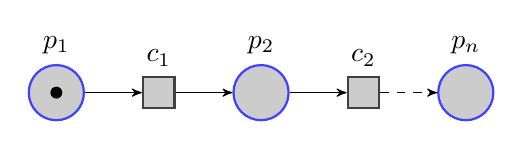
\begin{tikzpicture}[node distance=1.3cm,>=stealth',bend angle=45,auto]
    % Styles are from https://texample.net/tikz/examples/nodetutorial/
    \tikzstyle{place-time}=[circle,thick,draw=blue!75,fill=black!20,minimum size=7mm]
    \tikzstyle{transition}=[rectangle,thick,draw=black!75,
    fill=black!20,minimum size=4mm]

    \node [place-time,tokens=1] (p1) [label=above:$p_1$] {};
    \node [transition] (t1) [right of=p1,label=above:$c_1$] {};
    \node [place-time]          (p2) [right of=t1,tokens=0,label=above:$p_2$] {};
    \node [transition] (t2) [right of=p2,label=$c_2$] {};
    \node [place-time]          (pn) [right of=t2,tokens=0,label=above:$p_n$] {};

    \path (p1) edge [->] (t1);
    \path (t1) edge [->] (p2);
    \path (p2) edge [->] (t2);
    \path (t2) edge [->,dashed] (pn);

  \end{tikzpicture}
\caption{Petri net modeling the passage of time as observed by \glspl{app}}
\label{fig:petri-net-time}
\end{figure}

\paragraph{Transaction status change}

The status of a transaction changes multiple times after it has been sent to the node.
Transactions start out in the node's \emph{mempool}.
Then their status changes to \emph{tentatively confirmed} or to \emph{rejected}.
Finally, a transaction that is tentatively confirmed can revert back to \emph{mempool} or it can become \emph{permantently confirmed} when enough blocks have been added to make it irreversible.

For each of the four states of a transaction, there is one place in the petri net, as shown in \ref{fig:petri-net-txn}.
% TODO: Should probably use colored tokens here for different transactions that we can distinguish.

\begin{figure}
  \centering
  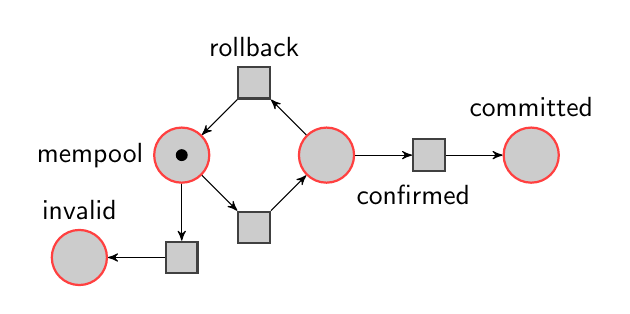
\begin{tikzpicture}[node distance=1.3cm,>=stealth',bend angle=45,auto]
    % Styles are from https://texample.net/tikz/examples/nodetutorial/
    \tikzstyle{place-status}=[circle,thick,draw=red!75,fill=black!20,minimum size=7mm]
    \tikzstyle{transition}=[rectangle,thick,draw=black!75,
    fill=black!20,minimum size=4mm]

    \node [place-status,tokens=1] (mempool)   [label=left:$\mathsf{mempool}$] {};
    \node [transition]     (confirm)   [below right of=mempool] {};
    \node [transition]     (rollback)   [above right of=mempool,label=above:$\mathsf{rollback}$] {};
    \node [place-status]          (confirmed) [below right of=rollback,tokens=0,label=below right:$\mathsf{confirmed}$] {};
    \node [transition]     (commit)    [right of=confirmed] {};
    \node [place-status]          (committed) [right of=commit,tokens=0,label=above:$\mathsf{committed}$] {};
    \node [transition]     (reject)  [below of=mempool] {};
    \node [place-status]          (invalid)  [left of=reject,label=$\mathsf{invalid}$] {};

    \path (mempool) edge [->] (confirm);
    \path (confirm) edge [->] (confirmed);
    \path (confirmed) edge [->] (rollback);
    \path (rollback) edge [->] (mempool);
    \path (confirmed) edge [->] (commit);
    \path (commit) edge [->] (committed);
    \path (mempool) edge [->] (reject);
    \path (reject) edge [->] (invalid);

  \end{tikzpicture}
\caption{Petri net for the status of transactions}
\label{fig:petri-net-txn}
\end{figure}

\paragraph{Address change}

The set of unspent outputs at an address is modified by transactions that spend and produce outputs.
Therefore, whenever the status of a transaction changes, the status of its inputs and outputs changes also.

We represent the outputs at each address with two petri nets, one for unspent outputs and one for spent outputs.
There is one place each for outputs that are in the mempool, tentatively confirmed, permantently confirmed, rejected.

% TODO: Think about how to do it properly. What level of detail do we need here? Maybe we don't need an extra petri net (address change is just a function of tx change). Or maybe we should include tx dependencies via their outputs as well.

\paragraph{Endpoint}

Users and other applications may call endpoints on the \gls{app}.
Endpoints are places $e_1, \ldots, e_n$ in the petri net (see \ref{fig:petri-net-endpoint}).

\begin{figure}
  \centering
  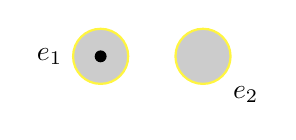
\begin{tikzpicture}[node distance=1.3cm,>=stealth',bend angle=45,auto]
    % Styles are from https://texample.net/tikz/examples/nodetutorial/
    \tikzstyle{place-endpoint}=[circle,thick,draw=yellow!75,fill=black!20,minimum size=7mm]
    \tikzstyle{transition}=[rectangle,thick,draw=black!75,
    fill=black!20,minimum size=4mm]

    \node [place-endpoint,tokens=1] (ep1) [label=left:$e_1$] {};
    \node [place-endpoint]          (ep2) [right of=ep1,label=below right:$e_2$] {};

  \end{tikzpicture}
\caption{Petri net for endpoints. The token in $e_1$ signifies that input is available to be consumed by this contract.}
\label{fig:petri-net-endpoint}
\end{figure}

\paragraph{Apps}

Given the places for time, transaction status, and endpoints we can describe \glspl{app} as sequences of transitions.
The states of the app are represented by places.
\ref{fig:plutus-app-net} shows a \gls{app} with three possible states, $s_1$, $s_2$ and $s_3$.
As soon as a transaction is confirmed, the state can progress from $s_1$ to $s_2$.

After that, endpoint $e_1$ becomes \emph{active}, meaning that the app can make progress as soon as input is provided. The next state depends on which of two possible events happens first: The endpoint being called by the user, or the clock reaching slot ten.

The app transitions (green) involve queries to the \gls{chain-index}, transaction submission, etc.
These requests are not shown in the petri net.
We still record their responses, however, in order to meet the replayability requirements (see \ref{req:app-synch} and \ref{req:app-reproducibility}).

\begin{figure}
  \centering
  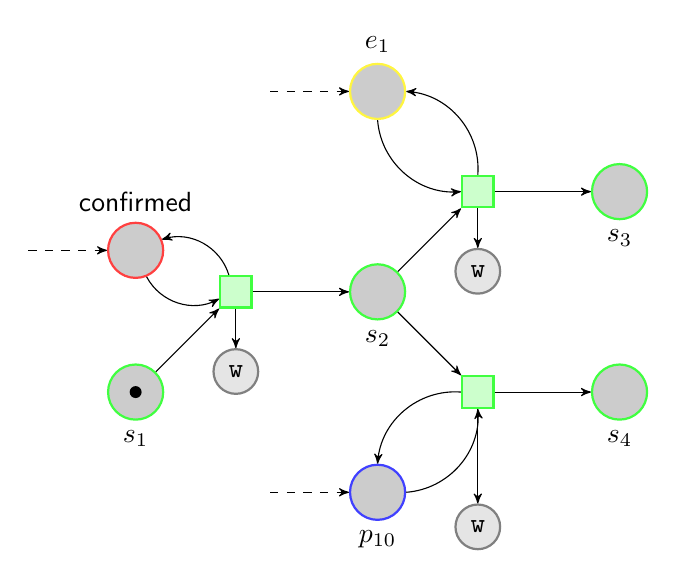
\begin{tikzpicture}[node distance=1.8cm,>=stealth',bend angle=45,auto]
    % Styles are from https://texample.net/tikz/examples/nodetutorial/
    \tikzstyle{place-endpoint}=[circle,thick,draw=yellow!75,fill=black!20,minimum size=7mm]
    \tikzstyle{place-status}=[circle,thick,draw=red!75,fill=black!20,minimum size=7mm]
    \tikzstyle{place-time}=[circle,thick,draw=blue!75,fill=black!20,minimum size=7mm]
    \tikzstyle{place-app}=[circle,thick,draw=green!75,fill=black!20,minimum size=7mm]
    \tikzstyle{place-writer}=[circle,thick,draw=black!50,fill=black!10,minimum size=4mm]
    \tikzstyle{transition-app}=[rectangle,thick,draw=green!75,fill=green!20,minimum size=4mm]

    \node [place-status]   (confirmed) [label=above:$\mathsf{confirmed}$]     {};
    \node [place-app]      (s1)        [below of=confirmed,tokens=1,label=below:$s_1$] {};
    \node [transition-app] (t1)        [above right of=s1]                    {};
    \node [place-writer]   (w1)        [below=0.5cm of t1] {\code{w}};

    \path (confirmed) edge [->,bend right] (t1);
    \coordinate[yshift=0,left=1cm of confirmed.west] (aux1);
    \path (aux1) edge [->,dashed] (confirmed);
    \path (t1) edge [->,bend right] (confirmed);
    \path (s1) edge [->] (t1);
    \path (t1) edge [->] (w1);

    \node [place-app]      (s2)        [right of=t1,label=below:$s_2$] {};
    \path (t1) edge [->] (s2);
    \node [transition-app] (t2) [above right of=s2] {};
    \node [place-writer]   (w2)        [below=0.5cm of t2] {\code{w}};
    \path (t2) edge [->] (w2);

    \node [transition-app] (t3) [below right of=s2] {};
    \node [place-writer]   (w3)        [below=1.2cm of t3] {\code{w}};
    \path (t3) edge [->] (w3);

    \node [place-app]      (s3)        [right of=t2,label=below:$s_3$] {};
    \path (s2) edge [->] (t2);
    \path (t2) edge [->] (s3);

    \node [place-endpoint] (e1) [above left of=t2,label=above:$e_1$] {};
    \coordinate[yshift=0,left=1cm of e1.west] (aux2);
    \path (aux2) edge [->,dashed] (e1);
    \path (e1) edge [->, bend right] (t2);
    \path (t2) edge [->, bend right] (e1);

    \node [place-app]      (s4)        [right of=t3,label=below:$s_4$] {};
    \path (s2) edge [->] (t3);
    \path (t3) edge [->] (s4);

    \node [place-time] (p10) [below left of=t3,tokens=0,label=below:$p_{10}$] {};
    \coordinate[yshift=0,left=1cm of p10.west] (aux3);
    \coordinate[yshift=0,right=1cm of p10.east] (aux4);
    \path (aux3) edge [->,dashed] (p10);
    \path (p10) edge [->, bend right] (t3);
    \path (t3) edge [->, bend right] (p10);
  \end{tikzpicture}
\caption{
  Petri net for an \gls{app} (green) that waits for a transaction to be confirmed and then waits for slot number ten to begin, or for user input.
  The app emits values of type \code{w} on every transition.
  }
\label{fig:plutus-app-net}
\end{figure}

\paragraph{Observable state}

\glspl{app} need to be able to notify the outside world of changes.
To this end, the application can emit values of some user-defined type \code{w} whenever one of its transition fires.
In the Haskell library, this is realised using the \code{Writer w} effect, with \code{Monoid w} constraint.
Clients of the \gls{app} can subscribe to receive updates whenever the accumulated total of all values changes.

\paragraph{Extensions}

There are some possible extensions of the basic model of apps and events.
For example, we could model an on-chain state machine (in a Plutus script) as a petri net.
Then we could describe the interactions of multiple \glspl{app-inst} interacting with that state machine, including possible race conditions.
The petri net model is simple, but it scales easily over multiple machines and contracts.

\section{Authoring: the Plutus Haskell SDK}
\label{sec:sdk}

Just like web applications, \glspl{app} have two separate components which are deployed in separate execution environments:
\begin{itemize}
\item \gls{on-chain} which is stored on the blockchain and executed during the validation of new transactions (similar to the server component of a web application), and
\item \gls{off-chain} code which is deployed to and executed on the client machine of a blockchain user with access to the user’s wallet (similar to the client portion of a web application running in a user’s web browser\footnote{
In fact, in other systems off-chain code often executes in a web browser as well!
})
\end{itemize}

Why is this decomposition necessary? The on-chain code contains the \gls{app}'s enforceable components.
It needs to enforce that only transactions that meet the enforceable obligations are successfully validated and added to the chain.
In other words, the integrity of a \gls{app} depends on the integrity of the on-chain code: thus we need to store it on the cryptographically immutable blockchain to prevent tampering.
Moreover, \glspl{slot-leader} need to execute on-chain code to check that it is in fact satisfied.

Conversely, the \gls{off-chain}, which submits new transactions to the chain for validation and inclusion, necessarily needs to run in close association with a contract user’s wallet.
After all, each transaction needs to be paid for with transaction fees, and a wallet is the only place where the necessary credentials are held (anything else would compromise the security of the funds).

Existing blockchains and their smart contract and dapp frameworks use separate languages for the \gls{on-chain} and \gls{off-chain} (in Ethereum, Solidity, and JavaScript), and they tend to invent new languages for the on-chain component (e.g., Solidity).
This comes with the same disadvantages as using different languages for the client and server components of web apps.
However, when new languages are invented the situation is even worse because of the enormous overhead involved in creating a new language, compilers and other tools, libraries, teaching material, and generally growing a new language community. We would like to avoid this (\cref{req:source-lang-conservatism}).

We overcome these problems by using Haskell for both \gls{on-chain} and \gls{off-chain} code.
This enables us to build on the existing Haskell ecosystem and to share datatypes and code between the two.
However, a downside of this approach is that GHC forms part of our compilation toolchain, which we do not control and which may change unexpectedly (this can make it hard to satisfy \cref{req:compilation-stability,req:compilation-reproducibility}, for example).

The \gls{plutus-sdk} is our library and tooling support for writing \glspl{app} --- both their \gls{on-chain} and their \gls{off-chain} together.

\subsection{Requirements}
\begin{requirement}[Conservatism]
\label{req:source-lang-conservatism}
Designing a new programming language is hard.
Designing a new \emph{source} programming language (one written by users directly) is even worse.
One must worry about syntax, tooling, build systems, libraries and their ecosystem, etc.

Ideally, we would like to avoid all this by reusing existing languages as much as possible.
\end{requirement}

\begin{requirement}[Lifting values at runtime]
\label{req:runtime-args}
The programs which we put on the chain cannot be entirely static (i.e. determined at \gls{off-chain} compile time).
It must be possible to parameterize them or partially generate them at runtime.

One reason for this is that we may want to configure our code.
For example, a crowdfunding \gls{app} might want to parameterize its \gls{on-chain} by the crowdfunding target, or the beneficiary of the funds.\footnote{
In some instances, one can get away with putting this information in the \gls{datum}.
The crowdfunding example is interesting because many people pay to the \gls{address} spontaneously, and the owner cannot control what those people put in the \glspl{datum}.
But they can control the \gls{address} people send to, and hence the \gls{script}.
So it is necessary to bake the parameters into the \gls{script} in this instance.
}
How can we parameterize a \gls{plutus-core} program?
One way is to write the program as a function, compile that function statically, then construct the argument at runtime and apply the program to the argument.
In pseudo-Haskell:
\begin{quote}
\begin{verbatim}
compile (\parameter -> ...) `apply` lift argument
\end{verbatim}
\end{quote}
\noindent This requires a way to ``lift'' a runtime value into an appropriate \gls{plutus-core} term so we can actually apply our compiled program to it.

This is just generally a very handy thing to be able to do and we want to be able to do it.
\end{requirement}

\begin{requirement}[Stability]
\label{req:compilation-stability}
When the \gls{plutus-core} program that makes up the \gls{on-chain} of a \gls{app} changes, so does its hash, and hence its \gls{address}.
This can be a big problem for applications: you cannot spend a \gls{script-output} without presenting a \gls{script} with \emph{exactly} that hash.
If your tooling won't produce such a \gls{script} anymore, then you can't get the money!

We, therefore, want our tooling to be as stable and deterministic as possible, so we don't change the output unnecessarily.

At the very least, we must not be sensitive to:
\begin{itemize}
\item The platform we are working on (linux/macos etc.)
\item Any random or mutable conditions
\end{itemize}
\end{requirement}

\begin{requirement}[Compilation reproducibility]
\label{req:compilation-reproducibility}
As discussed in \cref{req:compilation-stability}, if the output of compilation changes unexpectedly, then that can be a big problem.
But if the user changes their source or their tooling (e.g. their version of GHC), then that may just genuinely change the input to our compiler.

In this instance, there is not a great deal we can do at a technical level, except help people to build their applications reproducibly, so that
they can at least revert to previous states reliably.
\end{requirement}

\subsection{Haskell}

We need a source language for users to write \glspl{app} in.
We don't want to write our own one (\cref{req:source-lang-conservatism}), so we would really like to reuse an existing one.
We decided to use Haskell for a number of reasons:
\begin{itemize}
\item
  It is a powerful functional programming language.
\item
  It has an industrial-grade compiler, adequate tooling, and a good community and ecosystem.
\item
  It has good metaprogramming facilities.
\item
  We are familiar with it as a team and a company.
\end{itemize}

However, this means we need a way to compile (as a subsection of) a Haskell program into \gls{plutus-core}.
Our solution to this is \gls{plutus-tx}.

\subsection{Plutus Tx}
\label{sec:plutus-tx}

The \gls{plutus-tx} compiler compiles \gls{ghc-core} into \gls{plutus-core}.
That is, it takes Haskell after it has been desugared from its source representation into GHC's internal representation (\gls{ghc-core}), and compiles that further.
This approach allows us to support all of source Haskell while only having to deal with the much smaller \gls{ghc-core} language.

\subsubsection{Plugins for custom compilation}

GHC core-to-core plugins enable us to inject our own code including the \gls{plutus-tx} compiler into the GHC pipeline.
The \gls{plutus-tx} plugin,
\begin{enumerate}
\item locates \gls{ghc-core} fragments representing \gls{on-chain},
\item compiles them to \gls{plutus-core}, and
\item replaces each \gls{ghc-core} AST subtree representing \gls{on-chain} with an AST representing a serialised version of the generated \gls{plutus-core}.
\end{enumerate}

Overall, we end up with compiled \gls{off-chain} that embeds blobs of \gls{on-chain} in its serialised \gls{plutus-core} representation, ready to be submitted to the blockchain attached to transactions generated by the \gls{off-chain}.

There just seem to be two problems:
\begin{inparaenum}
\item how does the plugin identify on-chain code and
\item how do we ensure that the type of the serialised on-chain code lines up with the source code?\footnote{
\Gls{ghc-core} is a typed intermediate language; hence, any code transformation needs to be type-preserving.
}
\end{inparaenum}
We achieve this using a trick that to the best of our knowledge was first used in the \code{inline-java} package embedding Java into Haskell.
This package uses GHC plugins to extract type information at a Template Haskell splice point \autocite{inline-java-blog-post}.
The idea is to wrap the target Haskell code inside a splice of a Template Haskell function that inserts a marker around that AST fragment.

This function does not actually compile the AST of the target program fragment.
Instead, it inserts a marker function that is picked up by the \gls{plutus-tx} compiler injected with the plugin.
When the plugin runs, it finds the marker, compiles the code and inserts the serialized form back into the program.
By taking a little care over the types of our marker function, we can ensure that the expression in question remains well-typed at each stage of this process.

\subsubsection{Compiling GHC Core to Plutus Core}

Both \gls{ghc-core} and \gls{plutus-core} are extensions of \gls{system-f}.
\Gls{ghc-core} is a much more generous extension.
It adds mutually-recursive binding groups, algebraic data types, case expressions, coercions, and more.
In contrast, \gls{plutus-core}, as discussed in \cref{sec:plutus-core}, is much more minimal.

How do we deal with the extra features of \gls{ghc-core}?
First, we split the problem in half, by defining an intermediate language, \gls{plutus-ir} (see \cref{sec:plutus-ir}), which is much closer to \gls{ghc-core}.
Most of the theoretical complexity is therefore moved to the \gls{plutus-ir} compiler.

The remaining work of the \gls{plutus-tx} compiler is then to \emph{lower} the \gls{ghc-core} terms and types into their corresponding \gls{plutus-ir} variants, emitting errors as appropriate if we encounter features we do not support.

\subsubsection{Supporting Haskell's features}

As alluded to in the previous section, we do not support the entirety of Haskell.
Thanks to the design of GHC, we get a great deal for free, as we compile programs after they have been converted to \gls{ghc-core}, which means that most of the complex source-level features of Haskell have already been desugared into a smaller set of simpler features.

While we support most ``standard'' Haskell, there are quite a few things we do not support. A non-exhaustive list of features that we do not support is:
\begin{itemize}
\item Not implemented yet
  \begin{itemize}
  \item Mutually recursive datatypes (should be done by release)
  \end{itemize}
\item Incompatible with the design of \gls{plutus-core}
  \begin{itemize}
    \item \code{PolyKinds}, \code{DataKinds}, anything that moves towards ``Dependent Haskell''
  \end{itemize}
\item Technically difficult
  \begin{itemize}
  \item Literal patterns
  \end{itemize}
\item Requires access to function definitions (might be fixed with some GHC work)
  \begin{itemize}
  \item Function usage without \code{INLINEABLE} or \code{-fexpose-all-unfoldings}
  \item Typeclass dictionaries
  \end{itemize}
\item Use of coercions required
  \begin{itemize}
  \item GADTs
  \item \code{Data.Coerce}
  \item \code{DerivingVia}, \code{GeneralizedNewtypeDeriving}, etc.
  \end{itemize}
\item Assumes ``normal'' codegen
  \begin{itemize}
  \item FFI
  \item Numeric types other than integers
  \item Unlifted/\code{MagicHash} types
  \item Machine words, C strings, etc.
  \end{itemize}
\end{itemize}

\subsubsection{Strictness}
\label{sec:plutus-tx-strictness}

Haskell is a lazy language and \gls{plutus-core} is a strict language.
How can we compile a lazy language into a strict language efficiently?

The answer is that we handle this partially.
We generally compile Haskell as though it were strict, but the key exception is for non-value let-bindings.
That is, if we see a let-binding whose right-hand side is not a value (i.e. may evaluate further), then we compile it as a non-strict let-binding (see \cref{sec:pir-non-strict}).

Unfortunately, we have no proof that this approach is sound, which is an area for future work.

\subsubsection{Lifting values at runtime}
\label{sec:plutus-tx-lifting}

We are going to great lengths to compile \gls{on-chain} \glspl{validator} at \gls{off-chain} compile time.
However, we may also need to create some \gls{plutus-core} programs from \emph{runtime} values (\cref{req:runtime-args}).

Unfortunately, we cannot use the main \gls{plutus-tx} compiler for this: the \gls{plutus-tx} compiler turns Haskell \emph{programs} represented as \gls{ghc-core} into \gls{plutus-core}.
It cannot do anything with the \emph{runtime} representation of a Haskell value!

We, therefore, need to replicate what we \emph{would} do with the \gls{plutus-tx} compiler, but at runtime.
Fortunately, we can reuse the \gls{plutus-ir} compiler, which helps a lot.
We define a pair of typeclasses inspired by the Haskell typeclasses for ``lifting'' runtime values into metaprograms: \code{Lift} and \code{Typeable}.
Our typeclasses look something like this (\code{Term} and \code{Type} are the types for \gls{plutus-ir} terms and types; class constraints on the methods are omitted for simplicity):

\begin{quote}
\begin{verbatim}
class Lift a where
    lift :: (...) => a -> m (Term TyName Name ())

class Typeable a where
    typeRep :: (...) => Proxy a -> m (Type TyName ())
\end{verbatim}
\end{quote}

With some effort, we are able to generate instances for these with Template Haskell, so the burden on users is minimal.

Why do we output \gls{plutus-ir} here, rather than running the \gls{plutus-ir} compiler each time and just producing \gls{plutus-core}?
The reason is that the \gls{plutus-ir} compiler has some support for \emph{sharing} definitions, and it is important that programs generated from multiple calls to \code{lift} (e.g. from one implementation calling another, as is common) share the same definition of their shared types.

\subsection{Plutus IR}
\label{sec:plutus-ir}

\Gls{plutus-ir} is an intermediate language that sits between \gls{ghc-core} and \gls{plutus-core}.
Many of the core ideas are published in \textcite{peytonjones2019unraveling}, including the complex parts of compilation and the typesystem.

We give a high-level overview of the language here, further details can be found in the above reference.

\Gls{plutus-ir} is essentially \gls{plutus-core}, but with the addition of:
\begin{itemize}
\item Datatypes, including recursive and mutually recursive datatypes
\item Let terms, including recursive and mutually recursive bindings
\end{itemize}

Compiling recursive datatypes and recursive values are the two trickiest compilation problems, and are covered in \textcite{peytonjones2019unraveling}.

\subsubsection{Non-strict let bindings}
\label{sec:pir-non-strict}

\Gls{plutus-ir} has an additional feature which isn't discussed in \textcite{peytonjones2019unraveling}: non-strict let-bindings.
By default (and in the paper), let-bindings are \emph{strict}, meaning that the right-hand side of the binding is evaluated before the body of the term.

However, it is useful to support \emph{non-strict} let-bindings, particularly because these correspond more closely to the semantics of Haskell (see \cref{sec:plutus-tx-strictness}).
We can desugar these into strict let-bindings simply by inserting a \code{delay} on the binding right-hand side and a \code{force} at every use site.

\subsubsection{Optimization}

We do a small amount of optimization in the \gls{plutus-ir} compilation pipeline.
We don't want to do too much in case we make the generated code too unstable (\cref{req:compilation-stability}).

\paragraph{Dead code elimination}
\label{para:dead-code}

Dead code elimination is a straightforward optimization and is close to a clear win:
\begin{inparaenum}
\item it reduces code size,
\item it makes the code easier to read, and
\item it has no effect on semantics.
\end{inparaenum}

It is particularly helpful as the \gls{plutus-tx} compiler introduces definitions for all the builtins, some of which will be unused.

\subsubsection{Compilation}

The \gls{plutus-ir} compiler works via a series of small passes that eliminate individual features of \gls{plutus-ir} in turn, until the remaining program is pure \gls{plutus-core} and can simply be lowered into that AST type.

The passes are:
\begin{itemize}
\item Non-strict let-bindings into strict let-bindings by inserting thunks
\item Type bindings and datatypes into simple type and lambda abstractions
\item Recursive term bindings into non-recursive term bindings
  \begin{itemize}
  \item We do another dead code elimination pass (\cref{para:dead-code}) as this can introduce dead bindings.
  \end{itemize}
\item Non-recursive term bindings into lambda abstractions
\end{itemize}

\subsection{Cross-compilation}
\label{sec:cross-compilation}

To support \cref{req:app-dist}, we want to be able to compile \glspl{app} into easily redistributable \glspl{app-exe}.

The current approach is to target Javascript or WebAssembly as our format for distribution, and leverage cross-compilation of Haskell to actually produce the executables.

\subsubsection{Cross-compilers}

At the moment IOHK is working on two cross-compilation efforts:
\begin{description}
  \item[GHCJS] GHCJS is a Haskell cross-compiler that targets Javascript \autocite{ghcjs-repo}.
  \item[Asterius] Asterius is a Haskell cross-compiler that targets WebAssembly \autocite{asterius-repo}.
\end{description}

\noindent We may use either or both of these in the end.

\subsubsection{haskell.nix}

Cross-compilation of Haskell projects is not easy.
Neither of the major Haskell build tools (\code{cabal} and \code{stack}) support cross-compilation well.

To address this issue, IOHK has developed the \code{haskell.nix} framework for building Haskell projects using Nix \autocite{haskell-nix-repo}.
In addition to supporting cross-compilation well, Nix is well-suited to ensuring that builds are reproducible, which helps with \cref{req:compilation-reproducibility}.

\subsection{Developer tooling}
\label{sec:tooling}

Since the \gls{plutus-sdk} uses Haskell for development, there is much less need to create specialized development tooling, since generic Haskell tooling will work perfectly well.\footnote{
It is true that Haskell development tooling is generally considered to not be very good.
However, it is improving rapidly, and while it might be sensible for IOHK to contribute to the community's efforts on this front, that will be significantly less work than developing completely new tools.
}

It is possible that we may want to develop some tools, particularly for testing and visualization, but this has not been decided yet.


% Print the glossary
\printglossaries
\glsaddall

% Print the bibliography and include it in the TOC
\printbibliography[heading=bibintoc]

\end{document}
